\chapter{Modello standard}

\section{Rottura spontanea di simmetria (Wigner e Nambu-Goto)}

In \mq\ una simmetria è una mappa:
\begin{equation}
    \ket{\alpha} \quad \longrightarrow \quad \ket{\alpha^\prime} = U\, \ket{\alpha}
\end{equation}
tale per cui:
\begin{equation}
    \braket{\alpha}{\beta} = \braket{\alpha^\prime}{\beta^\prime}
\end{equation}
quindi $U$ dev'essere un operatore unitario. Inoltre ricordiamo che per il teorema di Noether ogni simmetria corrisponde una corrente conservata:
\begin{equation}
    \delta S \sim \int\dd^4 x\, \left(\partial_\mu j^\mu \right) = 0
\end{equation}
da cui ricaviamo la carica conservata:
\begin{equation}
    Q^a = \int\dd^4 x\, j^{0a}
\end{equation}
inoltre abbiamo che:
\begin{equation}
    \comm{H,Q^a} = 0
\end{equation}
e per questo possiamo esprimere:
\begin{equation}
    U = e^{i\, a^a\, Q^a}.
\end{equation}
Una simmetria può agire su una teoria in due modi diversi in base a come agisce sul vuoto: \textit{realizzazione alla Wigner} o \textit{realizzazione di Nambu-Goto}. Per Wigner abbiamo:
\begin{equation}
    U\, \ket{0} = \ket{0} \quad , \quad Q_0\, \ket{0} = 0
\end{equation}
pertanto tutto lo spettro è caratterizzato da multipletti del gruppo di simmetria ovvero di $Q_a$, quindi per esempio se abbiamo due stati degeneri allora:
\begin{equation}
    \ket{\alpha} = Q_a\, \ket{\alpha}.
\end{equation}
Per Nambu-Goto invece abbiamo:
\begin{equation}
    U\, \ket{0}\neq \ket{0}
\end{equation}
cioè il vuoto non è invariante, e con un abuso di notazione si dice che la \textit{simmetria è spontaneamente rotta} ($U$ continua a commutare con $H$).


\section{Rottura della simmetria e spettro di massa}

Consideriamo un campo reale scalare $\phi^a$ con $a=\{1,2\}$ e:
\begin{equation}
    \Lag = \frac{1}{2}\, \partial_\mu\phi^a\, \partial^\mu\phi^a - V(\phi^a)
\end{equation}
dunque per cui abbiamo:
\begin{equation}
    \Ham = \frac{1}{2}\left(\dot{\phi}^a\right)^2 + \frac{1}{2}\left(\nabla_i\phi^a\right)^2 + V(\phi^a)
\end{equation}
tuttavia la teoria dev'essere invariante di Poincarè (Lorentz e traslazioni nello spazio-tempo), quindi il vuoto della teoria è dato dalla condizione che estremizza del potenziale, cioè dobbiamo avere:
\begin{equation}
    \pdv{V}{\phi^a} = 0.
\end{equation}
Studiamo le conseguenze di queste due realizzazioni per lo spettro di massa della teoria. Nella lagrangiana non abbiamo scritto un termine di massa esplicito ma lo ritroviamo quando espandiamo in un intorno del vuoto:
\begin{equation}
    V(\phi^a) = V(\langle\phi^a\rangle) + \pdv{V}{\phi^a}\, (\phi^a - \langle\phi^a\rangle) + \frac{1}{2}\pdv[2]{V}{\phi^a}{\phi^b}\Bigg|_{\langle\phi\rangle}\, \left( \phi^a - \langle\phi^a\rangle \right)\, \left( \phi^b - \langle\phi^b\rangle \right)
\end{equation}
la derivata prima è nulla nel vuoto, il termine costante è l'energia di punto zero che può essere ignorata e dunque rimane solamente:
\begin{equation}
    M_{ab}^2 = \pdv[2]{V}{\phi^a}{\phi^b}\Bigg|_{\phi^a=\langle\phi^a\rangle}.
\end{equation}

Consideriamo una trasformazione:
\begin{equation}
    \delta\phi^a = R^a_b\, \phi^b
\end{equation}
di $SO(2)$, per la quale il potenziale trasforma con:
\begin{equation}
    \delta V = \pdv{V}{\phi^a}\, \delta\phi^a = \pdv{V}{\phi^a}\, R^a_b\, \phi^b.
\end{equation}
Tuttavia se ipotizziamo che $\Lag$ sia invariante di $SO(2)$, abbiamo che:
\begin{equation}
    \delta V = \left(\pdv{V}{\phi^a}\, R^a_b\, \phi_b\right)_{\langle\phi^b\rangle} = 0
\end{equation}
quindi:
\begin{align}
    \pdv{\phi^c}\left( \pdv{V}{\phi^a}\, R_b^a\, \phi^b \right)_{\langle\phi^b\rangle} &= \left( \pdv[2]{V}{\phi^a}{\phi^c}\, R_b^a\, \langle\phi^b\rangle + \pdv{V}{\phi^a}\, R_b^a\, \delta_c^b \right)_{\langle\phi^b\rangle} \\
    &= M_{ac}^2\, R^a_b\, \langle\phi_b\rangle \\
    &= 0.
\end{align}
Dunque, ricordando che la variazione del vuoto è:
\begin{equation}
    \delta\langle\phi^a\rangle = \alpha\, R_b^a\, \langle\phi^b\rangle
\end{equation}
possiamo avere:
\begin{itemize}
    \item La realizzazione alla Wigner se:
    \begin{equation}
        \delta\langle\phi^a\rangle R_a^b\, \langle\phi_b\rangle = 0
    \end{equation}
    che implica la \textit{preservazione del vuoto}:
    \begin{equation}
        U\, \ket{0} = \ket{0}
    \end{equation}
    che non dà informazioni aggiuntive sulle particelle.
    \item La realizzazione alla Nambu-Goto se:
    \begin{equation}
        \delta\langle\phi^a\rangle R_a^b\, \langle\phi_b\rangle \neq 0
    \end{equation}
    che implica la \textit{"rottura" del vuoto}:
    \begin{equation}
        U\, \ket{0} = \ket{0}
    \end{equation}
    in questo caso la matrice di massa $M^2_{ab}$ ha un autovalore nullo, dunque esiste sempre una particella a massa nulla, che prende il nome di \textbf{bosone di Goldstone}.
\end{itemize}


\section{Esempio di rottura della simmetria}

I riferimenti sono p. 348 del Peskin \cite{Peskin}. \\

Studiamo la lagrangiana:
\begin{equation}
    \Lag = \frac{1}{2}\sum_{b=1,2}\left(\partial_\mu\phi^b\right)\, \left(\partial^\mu\phi^b\right) - V(\phi^b) 
\end{equation}
in cui scegliamo:
\begin{equation}
    V(\phi^a) = \frac{\lambda}{4!}\left( \sum_{b=1,2}\frac{1}{2}\, \phi^b\, \phi^b - a^2 \right)^2.
\end{equation}
Passiamo ad un campo complesso:
\begin{equation}
    \phi = \frac{\phi^1 + i\, \phi^2}{\sqrt{2}}
\end{equation}
ed otteniamo:
\begin{equation}
    \Lag = \partial_\mu\phi\partial^\mu\phi^\dagger - \frac{\lambda}{4!}\, \left( \phi\phi^\dagger - a^2 \right)^2
    \label{eqn:5 lag con esempio rottura simm}
\end{equation}
e possiamo osservare che abbiamo un'invarianza di fase globale. Se vogliamo calcolare il vuoto della teoria dobbiamo studiare:
\begin{equation}
    \pdv{V}{\phi} = 0 \quad , \quad \pdv{V}{\phi^\dagger} = 0
\end{equation}
da cui otteniamo:
\begin{equation}
    \langle \phi \rangle = \langle \phi^\dagger \rangle = a
\end{equation}
oppure:
\begin{equation}
    \langle \phi \rangle = \langle \phi^\dagger \rangle = 0.
\end{equation}
Se abbiamo $a^2\leq 0$ abbiamo un'uncia soluzione:
\begin{equation}
    \langle \phi \rangle = 0
\end{equation}
dunque:
\begin{equation}
    M^2 = \begin{pmatrix}
        0 & -a^2 \\
        -a^2 & 0
    \end{pmatrix} \quad , \quad \text{det}M^2 \neq 0.
\end{equation}
Se $a^2>0$ abbiamo un massimo in $\langle \phi \rangle = 0$ ed un minimo in $\langle \phi \rangle = a$, infatti se andiamo a studiare la matrice di massa abbiamo:
\begin{align}
    &\partial_\phi^2 V = \overline{\phi}^2 \quad \longrightarrow \quad a^2 \\
    &\partial_{\overline{\phi}}^2 V = \phi^2 \quad \longrightarrow \quad a^2 \\
    &\partial_{\phi,\overline{\phi}}^2 V = 2\, \phi\, \overline{\phi} = 2\, \phi\, \overline{\phi} - a^2 \quad \longrightarrow\quad a^2
\end{align}
dunque abbiamo:
\begin{equation}
    M^2 = \begin{pmatrix}
        a^2 & a^2 \\
        a^2 & a^2
    \end{pmatrix} \quad , \quad \text{det}M^2 = 0
\end{equation}
quindi uno degli autovalori è nullo, dunque il vuoto rompe spontaneamente la simmetria, infatti in questo caso il vuoto realizza la simmetria alla Nambu-Goto.


\subsection{Sostituzione 1}

Prendendo (\ref{eqn:5 lag con esempio rottura simm}) studiamo:
\begin{equation}
    \phi = \rho\, e^{i\theta}
\end{equation}
per cui abbiamo:
\begin{align}
    &\partial_\mu\phi = \left( \partial_\mu\rho + i\rho\, \partial_\mu\theta \right)\, e^{i\theta} \\
    &\partial_\mu\phi^\dagger = \left( \partial_\mu\rho - i\rho\, \partial_\mu\theta \right)\, e^{-i\theta}
\end{align}
da cui:
\begin{equation}
    \Lag = \partial_\mu\rho\partial^\mu\rho + \rho^2\, \partial_\mu\theta\partial^\mu\theta - \frac{\lambda}{4!}\, (\rho^2 - a^2)^2
\end{equation}
il potenziale non dipende più da $\theta$ (che può essere il bosone di Goldstone) e per cui:
\begin{equation}
    \pdv{V}{\rho} = \frac{\lambda}{6}\, (\rho^2 - a^2)\, \rho = 0
\end{equation}
che implica:
\begin{align}
    &\langle\rho\rangle = 0 \qquad &&\text{(massimo)} \\
    &\langle\rho\rangle = \rho_0 = \pm a \qquad &&\text{(minimo)}.
\end{align}
Espandendo il potenziale intorno al vuoto, ignorando l'energia di punto zero, abbiamo:
\begin{align}
    V(\rho) &\approx \frac{1}{2}\, \pdv[2]{V}{\rho}\, (\rho - \rho_0)^2 \\
    &= \frac{\lambda}{6}\, a^2\, (\rho - \rho_0)^2.
\end{align}
Se poniamo $\xi = \rho - \rho_0$ otteniamo:
\begin{equation}
    \Lag = \partial_\mu\xi\partial^\mu\xi + (\xi + \rho_0)^2\, \partial_\mu\theta\partial^\mu\theta - \frac{\lambda}{6}\, a^2\, \xi^2 + \dots
\end{equation}
se trascuriamo anche i termini di accoppiamento (infatti per determinare lo spettro di massa ci bastano i termini quadratici) abbiamo che:
\begin{equation}
    \Lag = \partial_\mu\xi\partial^\mu\xi + \rho_0^2\, \partial_\mu\theta\partial^\mu\theta - \frac{\lambda}{6}\, a^2\, \xi^2 + \dots
\end{equation}
quindi $\theta$ è il bosone di Goldstone, mentre $\xi$ è un campo massivo. Infine, dobbiamo rinormalizzare i due campi:
\begin{equation}
    \xi \ \longrightarrow \ \frac{1}{\sqrt{2}}\, \xi \quad , \quad \rho_0\, \theta \ \longrightarrow\ \frac{1}{\sqrt{2}}\, \theta
\end{equation}
in questo modo otteniamo:
\begin{equation}
    \Lag = \frac{1}{2}\, \partial_\mu\xi\partial^\mu\xi + \frac{1}{2}\, \partial_\mu\theta\partial^\mu\theta - \frac{\lambda}{12}\, a^2\, \xi^2 + \dots
\end{equation}


\subsection{Sostituzione 2}

Ripartendo da (\ref{eqn:5 lag con esempio rottura simm}), ma trasliamo rispetto al vuoto:
\begin{equation}
    \phi = \frac{\xi + i\theta}{\sqrt{2}} + \langle\phi\rangle \quad , \quad \langle\phi\rangle = a
\end{equation}
in questo modo otteniamo:
\begin{align}
    \Lag &= \frac{1}{2}\, \partial_\mu\xi\, \partial^\mu\xi + \frac{1}{2}\, \partial_\mu\theta\, \partial^\mu\theta - \frac{\lambda}{4\cdot 4!}\, \left( \xi^2 + \theta^2 + 2\sqrt{2}\, a\xi \right)^2 \\
    &= \frac{1}{2}\, \partial_\mu\xi\, \partial^\mu\xi + \frac{1}{2}\, \partial_\mu\theta\, \partial^\mu\theta - \frac{\lambda}{4\cdot 4!}\, \left( \xi^4 + \theta^4 + 8\, a^2\, \xi^2 + 2\, \xi^2\, \theta^2 + 4\sqrt{2}\, a\, \xi^3 + 4\sqrt{2}\, a\, \xi\, \theta^2 \right)^2
\end{align}
dunque $\xi$ ha massa:
\begin{equation}
    m_\xi^2 = \frac{\lambda}{6}\, a^2
\end{equation}
mentre $\theta$ resta massless e rappresenta il bosone di Goldstone.

\paragraph{Osservazione}Dopo aver fatto una traslazione rispetto al vuoto, se volessimo fare una traslazione di fase infinitesima per mantenere la lagrangiana invariante dovremmo studiare una trasformazione non lineare. \textcolor{red}{forse a lezione (21) si fa un esempio.}


\section{Fotone massivo tramite Goldstone}

Consideriamo la simmetria $U(1)$ (di fase) locale:
\begin{equation}
    \Lag = -\frac{1}{4}\, F_{\mu\nu}\, F^{\mu\nu} + \left(D_\mu\phi\right)^\dagger\, \left(D^\mu\phi\right) - V(\phi\, \phi^\dagger)
\end{equation}
in cui abbiamo:
\begin{equation}
    D_\mu\phi = \left( \partial_\mu + ie\, A_\mu \right)\, \phi
\end{equation}
e studiamo:
\begin{equation}
    V(\phi\, \phi^\dagger) = \frac{\lambda}{4!}\, \left( \phi\, \phi^\dagger - a^2 \right)^2
\end{equation}
con $\langle\phi\rangle = \langle\phi^\dagger\rangle = a$ e $a^2>0$. Osserviamo che i gradi di libertà totali sono 4 (due dallo scalare complesso $\phi$ e due dal fotone $A$).


\subsection{Sostituzione}

Consideriamo $\phi = \rho\, e^{i\theta}$, per cui:
\begin{align}
    D_\mu\phi &= \Big( \partial_\mu\rho + i\rho\, \partial_\mu\theta + ie\, A_\mu\, \rho \Big)\, e^{i\theta} \\
    &= \Big( \partial_\mu\rho + i\rho(\partial_\mu\theta + e\, A_\mu) \Big)\, e^{i\theta}
\end{align}
e conseguentemente:
\begin{align}
    \Lag &= -\frac{1}{4}\, F_{\mu\nu}\, F^{\mu\nu} + \partial_\mu\rho\partial^\mu\rho + \rho^2\, \left(\partial_\mu\theta + e\, A_\mu\right)^2 - \frac{\lambda}{4!}\, (\rho^2 - a^2)^2 \\
    &= -\frac{1}{4}\, F_{\mu\nu}\, F^{\mu\nu} + \partial_\mu\rho\partial^\mu\rho + \rho^2\, e^2\, A_\mu\, A^\mu - \frac{\lambda}{4!}\, (\rho^2 - a^2)^2
\end{align}
in cui nell'ultimo passaggio abbiamo fatto la trasformazione di gauge:
\begin{equation}
    A_\mu^\prime = A_\mu + \frac{1}{e}\, \partial_\mu\theta
\end{equation}
in questo modo il bosone di Goldestone è stato riassorbito nel fotone che ha acquistato massa:
\begin{equation}
    m_A^2 = 2\, a^2\, e^2.
\end{equation}
Espandendo intorno al vuoto ponendo:
\begin{equation}
    \xi = \rho - \rho_0
\end{equation}
in cui:
\begin{equation}
    \langle\rho\rangle = \rho_0 = \pm a
\end{equation}
otteniamo:
\begin{align}
    \Lag &= -\frac{1}{4}\, F_{\mu\nu}\, F^{\mu\nu} + \partial_\mu\xi\partial^\mu\xi + (\xi + \rho_0)^2\, e^2\, A_\mu\, A^\mu - \frac{\lambda}{4!}\, \Big( (\xi + \rho_0)^2 - \rho_0^2 \Big)^2 \\
    &= -\frac{1}{4}\, F_{\mu\nu}\, F^{\mu\nu} + \partial_\mu\xi\partial^\mu\xi + (\xi^2 + 2\, \rho_0\, \xi + \rho_o^2)\, e^2\, A_\mu\, A^\mu - \frac{\lambda}{4!}\, \Big[ \xi^2 + 2\, \rho_0\, \xi \Big]^2 \\
    &= -\frac{1}{4}\, F_{\mu\nu}\, F^{\mu\nu} + \partial_\mu\xi\partial^\mu\xi + \rho_0^2\, e^2\, A_\mu\, A^\mu - \frac{\lambda}{6}\, \rho_0^2\, \xi^2 + \Lag_{int}
\end{align}
in cui poniamo:
\begin{equation}
    \Lag_{int} = \Big( \xi^2 + 2\rho_0\, \xi \Big)\, e^2\, A_\mu\, A^\mu - \frac{\lambda}{4!}\, \Big[ \xi^4 + 4\rho_0\, \xi^3 \Big].
\end{equation}
Infine, dobbiamo rinormalizzare:
\begin{equation}
    \xi \quad \longrightarrow \quad \frac{1}{\sqrt{2}}\, \xi
\end{equation}
e sostituiamo $\rho_0^2 = a^2$, così otteniamo:
\begin{equation}
    \Lag = -\frac{1}{4}\, F_{\mu\nu}\, F^{\mu\nu} + \frac{1}{2}\, \partial_\mu\xi\partial^\mu\xi + a^2\, e^2\, A_\mu\, A^\mu - \frac{\lambda}{12}\, a^2\, \xi^2 + \Lag_{int}
\end{equation}
dunque, che sta descrivendo un campo $\xi$ reale con la stessa massa vista in precedenza:
\begin{equation}
    m_\xi^2 = \frac{\lambda}{6}\, a^2
\end{equation}
ed un campo vettoriale massivo con:
\begin{equation}
    M_A^2 = 2\, a^2\, e^2.
\end{equation}

\paragraph{Osservazione.}Il risultato assomiglia alla lagrangiana di Proca (i termini quadratici sono uguali, ma i termini di interazione sono diversi) ma sta volta è rinormalizzabile; la rottura spontanea della simmetria preserva i gradi di libertà e li riorganizza: un grado di libertà appartiene a $\xi$ (particella di Higgs) e 3 appartengono al bosone massivo $A$, in più la trasformazione di gauge equivale a inglobare il bosone di Goldstone dentro $A$ e in particolare la polarizzazione longitudinale di $A$ coincide con il bosone di Goldstone.

\textbf{Nota.} Non si può fare un discorso analogo con il campo spinoriale perché dovremmo fissare l'invarianza per rotazione e quindi l'invarianza di Lorentz/Poincaré!


\section{La lagrangiana di Fermi}

Per la QED sappiamo di avere:
\begin{equation}
    \Lag_{QED} = \overline{\psi}\, \left( i\slashed{\partial} - e\, \slashed{A} + m \right)\, \psi - \frac{1}{4}\, F_{\mu\nu}\, F^{\mu\nu}
\end{equation}
ma le particelle possono interagire anche tramite la forza debole e la forza forte. La descrizione di Fermi per la forza debole descrive l'interazione tramite la corrente:
\begin{equation}
    \Lag_F = \frac{G_F}{\sqrt{2}}\, J^\mu\, J_\mu^\dagger \qquad \text{con}\quad J^\mu = L^\mu + H^\mu
\end{equation}
con all'interno i termini che chiamiamo \textbf{corrente leptonica} e \textbf{corrente adronica}, la costante di Fermi è:
\begin{equation}
    G_F = 1.166\cdot 10^{-5}\, \unit{\giga\eV^{-2}}.
\end{equation}
Le due correnti vengono costruite in analogia con la QED:
\begin{equation}
    L^\mu \sim H^\mu\sim \overline{\psi}\, \left( G_V\, V^\mu - G_A\, A^\mu \right)\, \psi
\end{equation}
dove $V$ è la corrente vettoriale ed $A$ è la corrente assiale $A^\mu \sim \gamma^\mu\, \gamma_5$, il fatto che ci sia $V-A$ è legato al fatto che solo la componente Left partecipa all'interazione.

Notiamo che siccome vale:
\begin{equation}
    (\gamma_5)^\dagger = \gamma_5 \quad , \quad (\gamma^\mu)^\dagger = \gamma^0\, \gamma^\mu\, \gamma^0 \quad ,\quad (\gamma^0)^2 = \mathbb{1}
\end{equation}
abbiamo che:
\begin{align}
    j_\mu &= \overline{\chi}\, \gamma_\mu\, (1-\gamma_5)\, \xi \\
    \Longrightarrow \quad j_\mu^\dagger &= \xi^\dagger\, \left(1-\gamma_5^\dagger\right)\, \gamma_\mu^\dagger\, (\gamma^0)^\dagger\, \chi \\
    &= \xi^\dagger\, (1-\gamma_5)\, (\gamma^0\, \gamma_\mu)\, \chi \\
    &= \xi^\dagger\, (\gamma^0\, \gamma\mu)\, (1-\gamma_5)\, \chi \\
    &= \overline{\xi}\, \gamma_\mu\, (1-\gamma_5)\, \chi.
\end{align}

Le costanti $G_V$ , $G_A$ sono diverse in base al tipo di particella che interagisce, sperimentalmente si trova $G_V = G_A = 1$ per le particelle elementari/puntiformi. Tuttavia questa teoria è valida anche per protoni e neutroni (entro un certo range di energia) con $G_V\approx 1$, $G_A=\alpha\approx 1.24$.

Scriviamo:
\begin{multline}
    \Lag_F \sim \frac{G_F}{\sqrt{2}}\, \bigg( \overline{\nu}_e\, \gamma^\mu\, (1-\gamma_5)\, \nu_e \bigg)\, \bigg( \overline{e}\, \gamma_\mu\, (1-\gamma_5)\, e \bigg) + \\
    + \frac{G_F}{\sqrt{2}}\, \bigg( \overline{p}\, \gamma^\mu\, (1-\alpha\gamma_5)\, n \bigg)\, \bigg( \overline{e}\, \gamma_\mu\, (1-\gamma_5)\, \nu \bigg)
\end{multline}
dove $\nu_e$ è lo spinore di Dirac per il neutrino elettronico, mentre $e$ è il campo di Dirac per l'elettrone, e la presenza della $\gamma_5$ esprime il fatto che non viene conservata la parità.

Se facciamo l'analisi dimensionale:
\begin{equation}
    [S] = [\Lag]\cdot L^4 = 1
\end{equation}
dunque:
\begin{itemize}
    \item Per gli spinori:
    \begin{equation}
        \Lag = \overline{\psi}\, \left( i\slashed{\partial} - m \right)\, \psi
    \end{equation}
    dunque:
    \begin{equation*}
        [\Lag] \sim [\psi]^2\, L^{-1} = L^{-4}
    \end{equation*}
    che implica:
    \begin{equation*}
        [\psi] = L^{-3/2}.
    \end{equation*}
    \item Per gli sclari:
    \begin{equation}
        \Lag = \frac{1}{2}\, (\partial_\mu\phi)\, (\partial^\mu\phi) - \frac{1}{2}\, m^2\, \phi^2
    \end{equation}
    e per i bosoni vettori:
    \begin{equation}
        \Lag = -\frac{1}{4}\, F^{\mu\nu}\, F_{\mu\nu}
    \end{equation}
    dunque:
    \begin{equation*}
        [\Lag] \sim [\phi]^2\, L^{-2} = L^{-4}
    \end{equation*}
    che implica:
    \begin{equation*}
        [\phi] = [ A_\mu ] =  L^{-1}.
    \end{equation*}
\end{itemize}
Ciò implica che la costante di accoppiamento $g=e$ della QED sia adimensionale:
\begin{equation}
    [\Lag] = [g]\, [\psi]^2\, [A_\mu] = [g]\, L^{-3}\, L^{-1} = L^{-4} \quad \Longrightarrow \quad [g] = 1.
\end{equation}
Mentre nella lagrangiana di Fermi:
\begin{equation}
    [\Lag] = [G_F]\, [\psi]^4 = [G_F]\, L^{-6} = L^{-4}
\end{equation}
ovvero:
\begin{equation}
    [G_F] = L^2 = M^{-2}.
\end{equation}
Vedremo che $G_F$ è dimensionale perché nasconde al suo interno il propagatore dei bosoni vettori a basse energia.


\subsection{Validità della teoria di Fermi}

Nel limite di basse energie la teoria di Fermi è valida, mentre ad alte energie $\sigma$ cresce con l'energia del centro di massa e la teoria non è più unitaria. Se studiamo l'interazione, vedi in particolare il processo:
\begin{equation*}
    e + \overline{\nu}_e \quad \longrightarrow \quad e + \overline{\nu}_e
\end{equation*}
nel diagramma in figura \ref{fig:5 raff validità Fermi}, allora abbiamo 4 gambe esterne e l'elemento di matrice $S$ ridotta è:
\begin{equation}
    M = -i\, \frac{G_F}{\sqrt{2}}\, \Big( \overline{\nu}_2\, \gamma^\mu\, (1-\gamma^5)\, \nu_4 \Big)\, \Big( \overline{u}_3\, \gamma_\mu\, (a-b\, \gamma_5)\, u_1 \Big)
\end{equation}
\begin{figure}[ht!]
    \centering
    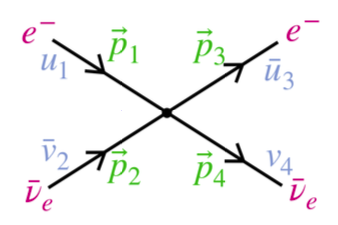
\includegraphics[width=0.6\textwidth]{Figure/5-SM/validità Fermi.png}
    \caption{Raffigurazione processo $e + \overline{\nu}_e\longrightarrow e + \overline{\nu}_e$.}
    \label{fig:5 raff validità Fermi}
\end{figure}

\noindent e dunque:
\begin{align}
    |\mathcal{M}|^2 &= \frac{1}{4}\sum_{spin}|M|^2 \\
    &= \frac{G_F^2}{8}\sum_{spin} \Big( \overline{\nu}_2\, \gamma^\mu\, (1-\gamma^5)\, \nu_4 \Big)\, \Big( \overline{\nu}_4\, \gamma^\nu\, (1-\gamma^5)\, \nu_2 \Big)\, \cross \notag \\
    &\qquad \cross \Big( \overline{u}_3\, \gamma_\mu\, (a-b\, \gamma_5)\, u_1 \Big)\, \Big( \overline{u}_1\, \gamma_\nu\, (a-b\, \gamma_5)\, u_3 \Big) \\
    &= \frac{G_F^2}{8}\, \Tr{(\slashed{p}_1 + m_e)\, \gamma_\nu\, (a - b\, \gamma_5)\, (\slashed{p}_3 + m_e)\, \gamma_\mu\, (a - b\, \gamma_5)}\, \cross \notag \\
    &\qquad \cross \Tr{(\slashed{p}_4 - m_\nu)\, \gamma^\nu\, (1 -  \gamma_5)\, (\slashed{p}_2 - m_\nu)\, \gamma^\mu\, (1 - \gamma_5)} \\
    &\approx \frac{G_F}{8}\, \Tr{(\slashed{p}_1)\, \gamma_\nu\, (a - b\, \gamma_5)\, (\slashed{p}_3)\, \gamma_\mu\, (a - b\, \gamma_5)}\, \cross \notag \\
    &\qquad \cross \Tr{(\slashed{p}_4)\, \gamma^\nu\, (1 -  \gamma_5)\, (\slashed{p}_2)\, \gamma^\mu\, (1 - \gamma_5)} \\
    &= \frac{G_F^2}{8}\, (p_1)^\alpha\, (p_3)^\beta\, (p_2)_\rho\, (p_4)_\sigma\, \Tr{\gamma_\alpha\, \gamma_\nu\, \gamma_\beta\, \gamma_\mu\, (a - b\, \gamma_5)^2}\, \cross \notag \\
    &\qquad \cross \Tr{\gamma^\sigma\, \gamma^\nu\, \gamma^\rho\, \gamma^\mu\, (1 - \gamma_5)^2} \\
    &= \frac{G_F^2}{8}\, (p_1)^\alpha\, (p_3)^\beta\, (p_2)_\rho\, (p_4)_\sigma\, \Tr{\gamma_\alpha\, \gamma_\nu\, \gamma_\beta\, \gamma_\mu\, (a^ + b^2 - 2a\, b\, \gamma_5)}\, \cross \notag \\
    &\qquad \cross \Tr{\gamma^\sigma\, \gamma^\nu\, \gamma^\rho\, \gamma^\mu\, (2 - 2\, \gamma_5)} \\
    &= 4\, G_F^2\, (p_1)^\alpha\, (p_3)^\beta\, (p_2)_\rho\, (p_4)_\sigma\, \Big[ (a^2 + b^2)\, \big( \eta_{a\nu}\, \eta_{\beta\mu} + \eta_{\alpha\mu}\, \eta_{\beta\nu} - \eta_{\alpha\beta}\, \eta_{\mu\nu} \big) + \notag \\
    &\qquad + 2iab\, \varepsilon_{\alpha\nu\beta\mu} \Big]\, \Big[ \eta^{\sigma\nu}\, \eta^{\rho\mu} + \eta^{\sigma\mu}\, \eta^{\rho\nu} - \eta^{\sigma\rho}\, \eta_{\mu\nu} + i\varepsilon^{\sigma\nu\rho\mu} \Big]
\end{align}
possiamo analizzare i termini separatamente:
\begin{align*}
    &\Big( \eta^{\sigma\nu}\, \eta^{\rho\mu} + \eta^{\sigma\mu}\, \eta^{\rho\nu} - \eta^{\sigma\rho}\, \eta_{\mu\nu} \Big)\, \Big( \eta_{a\nu}\, \eta_{\beta\mu} + \eta_{\alpha\mu}\, \eta_{\beta\nu} - \eta_{\alpha\beta}\, \eta_{\mu\nu} \Big) = 2\, \Big( \delta_\alpha^\sigma\, \delta_\beta^\rho + \delta_\alpha^\rho\, \delta_\beta^\sigma \Big) \\
    &\varepsilon^{\sigma\nu\rho\mu}\, \varepsilon_{\alpha\nu\beta\mu} = \varepsilon^{\mu\nu\rho\sigma}\, \varepsilon_{\mu\nu\alpha\beta} = -2\, \Big( \delta^\rho_\alpha\, \delta_\beta^\sigma - \delta_\alpha^\sigma\, \delta_\beta^\rho \Big) = 2\, \Big( \delta_\alpha^\sigma\, \delta_\beta^\rho - \delta^\rho_\alpha\, \delta_\beta^\sigma \Big) \\
    &\big( \eta_{a\nu}\, \eta_{\beta\mu} + \eta_{\alpha\mu}\, \eta_{\beta\nu} - \eta_{\alpha\beta}\, \eta_{\mu\nu} \big)\, \varepsilon^{\sigma\nu\rho\mu} = \big( \eta^{\sigma\nu}\, \eta^{\rho\mu} + \eta^{\sigma\mu}\, \eta^{\rho\nu} - \eta^{\sigma\rho}\, \eta_{\mu\nu} \big)\, \varepsilon_{\alpha\nu\beta\mu} = 0
\end{align*}
in cui l'ultima equazione è dovuta al fatto che $\varepsilon$ è anti-simmetrico per scambio di $\mu$, $\nu$, mentre il termine tra parentesi è simmetrico. Continuando i conti:
\begin{align}
    &= 8\, G_F^2\, (p_1)^\alpha\, (p_3)^\beta\, (p_2)_\rho\, (p_4)_\sigma\, \Big[ (a^2 + b^2)\, \Big( \delta_\alpha^\sigma\, \delta_\beta^\rho + \delta_\alpha^\rho\, \delta_\beta^\sigma \Big) - \notag \\
    &\qquad - 2ab\, \Big( \delta_\alpha^\sigma\, \delta_\beta^\rho - \delta^\rho_\alpha\, \delta_\beta^\sigma \Big) \Big] \\
    &= 8\, G_F^2\, \Big[ (a^2 + b^2 - 2ab)\, (p_1\cdot p_4)\, (p_2\cdot p_3) + \notag \\
    &\qquad + (a^2 + b^2 + 2ab)\, (p_1\cdot p_2)\, (p_3\cdot p_4) \Big] \\
    &= 2\, G_F^2\, \Big[ (a - b)^2\, u^2 + (a + b)^2\, s^2 \Big] \\
    &= 2\, G_F^2\, s^2\, \left[ \frac{1}{4}\, (a-b)^2\, (1 + \cos\theta)^2 + (a+b)^2 \right].
\end{align}
La sezione d'urto totale è:
\begin{align}
    \sigma &= \frac{1}{32\pi\, s}\int\dd(\cos\theta)\, |\mathcal{M}|^2 \\
    &= \frac{2\, G_F^2\, s}{32\, s}\, f(a,b) \\
    &\propto s = (p_1 + p_2)^2
\end{align}
dunque, questa teoria non è consistente ad alte energie perché le probabilità crescono in maniera indefinita, tuttavia è una buona approssimazione ad energia dell'ordine dell'energia di Fermi. L'unica dipendenza del momento in questa teoria viene fuori dalla media sulle polarizzazioni, per avere un andamento più ragionevole bisogna introdurre delle particelle che mediano l'interazione, tuttavia queste interazioni sono a corto raggio ($\sim 10^{-15}\ \unit{\meter}$), quindi non possiamo usare i fotoni come nella QED ma dobbiamo usare una particella massiva e il potenziale di Yukawa:
\begin{equation}
    V \sim \frac{1}{r}\, e^{-mr}
\end{equation}
dove $m$ è la massa della particella. Quindi dobbiamo introdurre un campo massivo che si accoppi con la corrente di Fermi:
\begin{equation}
    j_\mu\, B^\mu
\end{equation}
dove il campo $B$ ha un propagatore:
\begin{equation}
    \frac{i}{p^2 + m_B^2}
\end{equation}
e ciò fa in modo che la probabilità non cresca troppo ad alte energie, mentre a basse energie il campo $B$ non si propaga:
\begin{equation}
    \frac{1}{p^2 + m_B^2} \approx \frac{1}{m_B^2}.
\end{equation}
Si potrebbe pensare di introdurre un campo vettore massivo usando la lagrangiana di Proca:
\begin{equation}
    \Lag_P = -\frac{1}{4}\, F_{\mu\nu}\, F^{\mu\nu} + \frac{m_B^2}{2}\, B_\mu\, B^\mu
\end{equation}
che però non è invariante di gauge e questo fa si che la teoria non sia rinormalizzabile; per evitare questo problema si usa il \textit{meccanismo di Higgs}.


\section{Termini cinetici di Yang-Mills rispetto ad generatori}

Il termine di Yang-Mills è dato da $SU(3)_C \cross SU(2)_{I_3} \cross U(1)_Y$ con numeri quantici di colore $(C)$, isospin $(I_3)$ e ipercarica $(Y)$. Il gruppo $SU(3)$ descrive le interazioni di QCD tra i quark mediati dai gluoni, mentre $SU(2) \cross U(1)$ descrivono le interazioni eletteodeboli mediate dai bosoni $W_\mu^\pm$ (corrente debole carica), $Z_\mu$ (corrente debole neutra) e $A_\mu$ (corrente elettromagnetica).

Introduciamo inoltre le costanti di accoppiamento $g_3$, $g_2$, $g_1$, rispettivamente per l'interazione di colore $SU(3)_C$, l'interazione di isospin $SU(2)_{I_3}$ e l'interazione di ipercarica $U(1)_Y$.

Per il gruppo $SU(3)_C$ abbiamo i generatori:
\begin{equation}
    T^B = \frac{1}{2}\, \lambda^B \quad B\in\{1,\dots,8\}
\end{equation}
in cui $\lambda$ sono le \textbf{matrici di Gell-Mann-Low} ed i bosoni vettori sono i gluoni: $G_\mu^B$.

Il termine cinetico per la QCD è:
\begin{equation}
    \Lag_{QCD} = -\frac{1}{4}\sum_{B=1}^8 G_{\mu\nu}^B\, G^{\mu\nu B}
\end{equation}
che in realtà non utilizzeremo, ma l'abbiamo citata solo per completezza, e in cui definiamo:
\begin{equation}
    G_{\mu\nu}^B = \partial_\mu G_\nu^B - \partial_\nu G_\mu^B - g_3\, f^{BCD}\, G_\mu^C\, G_\nu^D.
\end{equation}

Per il gruppo $SU(2)_{I_3}$ abbiamo i generatori:
\begin{equation}
    T^a = \frac{1}{2}\, \sigma^a \quad a\in\{1,2,3\}
\end{equation}
in cui $\sigma$ sono le \textbf{matrici di Pauli} ed i bosoni vettori sono: $W_\mu^a$.

Il termine cinetico è:
\begin{equation}
    \Lag_{2} = -\frac{1}{4}\sum_{a=1}^3 W_{\mu\nu}^a\, G^{a\mu\nu}
\end{equation}
cui definiamo:
\begin{equation}
    W_{\mu\nu}^a = \partial_\mu W_\nu^a - \partial_\nu W_\mu^a - g_2\, \varepsilon^{abc}\, W_\mu^b\, W_\nu^c.
\end{equation}

Per il gruppo $U(1)_{Y}$ abbiamo un unico generatore (l'identità) ed un bosone vettore $B_\mu$. Il termine cinetico è:
\begin{equation}
    \Lag_1 = -\frac{1}{4}\, B_{\mu\nu}\, B^{\mu\nu}
\end{equation}
in cui definiamo:
\begin{equation}
    B_{\mu\nu} = \partial_\mu B_\nu - \partial_\nu B_\mu.
\end{equation}















\section{Trasformazione di carica e di parità}

Ricordiamo ancora che $\sigma^\mu = (\mathbb{1},\vec{\sigma})$, $\overline{\sigma}^\mu = (\mathbb{1},-\vec{\sigma})$ e che nella rappresentazione di Weyl:
\begin{equation}
    \gamma^\mu = \begin{pmatrix}
        0 & \sigma^\mu \\
        \overline{\sigma}^\mu & 0
    \end{pmatrix}
\end{equation}
ma anche che, nella stessa rappresentazione:
\begin{equation*}
    \gamma^0 = \begin{pmatrix}
        0 & \mathbb{1} \\
        \mathbb{1} & 0
    \end{pmatrix} \qquad \gamma^i = \begin{pmatrix}
        0 & \sigma^i \\
        -\sigma^i & 0
    \end{pmatrix} \qquad \gamma_5 = \begin{pmatrix}
        \mathbb{1} & 0 \\
        0 & -\mathbb{1}  
    \end{pmatrix} \qquad C = \begin{pmatrix}
        i\sigma^2 & 0 \\
        0 & -i\sigma^2
    \end{pmatrix}.
\end{equation*}
Mentre in quella di Dirac:
\begin{equation*}
    \gamma^0 = \begin{pmatrix}
        \mathbb{1} & 0 \\
        0 & -\mathbb{1}
    \end{pmatrix} \qquad \gamma^i = \begin{pmatrix}
        0 & \sigma^i \\
        -\sigma^i & 0
    \end{pmatrix} \qquad \gamma_5 = \begin{pmatrix}
        0 & \mathbb{1} \\
        \mathbb{1} & 0
    \end{pmatrix} \qquad C = \begin{pmatrix}
        0 & -i\sigma^2 \\
        -i\sigma^2 & 0
    \end{pmatrix}.
\end{equation*}
La parità ($P$) in generale agisce come:
\begin{equation}
    \psi(t,\vec{x}) \quad \overset{P}{\longrightarrow}\quad \psi^P(t,\vec{x}) = \gamma^0\, \psi(t,-\vec{x}).
\end{equation}
La coniugazione di carica è:
\begin{equation}
    C = i\gamma^0\, \gamma^2 = -i\gamma^2\, \gamma^0
\end{equation}
e in generale agisce come:
\begin{equation}
    \psi \quad \overset{C}{\longrightarrow}\quad \psi^C = \mathcal{C}\, \psi\, \mathcal{C}^\dagger
\end{equation}
in base al tipo di campo a cui lo applichiamo abbiamo una trasformazione diversa rispetto $C$. Vediamo i deiversi casi.

\paragraph{Spinore chiriale.}La coniugazione di carica agisce come:
\begin{equation}
    \psi \quad \overset{C}{\longrightarrow}\quad \psi^C = \eta_{C}\, C(\overline{\psi})^T
\end{equation}
ovvero:
\begin{align}
    \psi = \begin{pmatrix}
        \psi_L \\
        \psi_R
    \end{pmatrix} \quad \overset{C}{\longrightarrow}\quad \psi^C &= \eta_{C}\, C(\overline{\psi})^T \\
    &= \eta_C\, C\, \gamma^0\, \psi^* \\
    &= -i\eta_C\, \gamma^2\, \psi^* \\
    &= \eta_C\, \begin{pmatrix}
        0 & -i\sigma^2 \\
        i\sigma^2 & 0
    \end{pmatrix}\, \begin{pmatrix}
        \psi_L^* \\
        \psi_R^*
    \end{pmatrix} \\
    &= \eta_C\, \begin{pmatrix}
        -i\sigma^2\, \psi_L^*(t,-\vec{x}) \\
        +i\sigma^2\, \psi_R^*(t,-\vec{x})
    \end{pmatrix}
\end{align}
per brevità richiediamo che la fase sia $\eta_C = 1$.

\paragraph{Scalare complesso.}La coniugazine restituisce:
\begin{equation}
    \Phi \quad \overset{C}{\longrightarrow}\quad \Phi^C = \Phi^*
\end{equation}
dunque per PC abbiamo:
\begin{align}
    \Phi = \begin{pmatrix}
        \phi_L \\
        \phi_R
    \end{pmatrix} \quad \overset{CP}{\longrightarrow}\quad \Phi^{CP} &= \Phi^*(t,-\vec{x}) = \begin{pmatrix}
        \phi_A^* \\
        \phi_B^*
    \end{pmatrix}.
\end{align}

\paragraph{Bosone vettore neutro.}Abbiamo:
\begin{equation}
    A_\mu \quad \overset{C}{\longrightarrow}\quad A_\mu^C = -A_\mu
\end{equation}
dunque per PC otteniamo:
\begin{align}
    &B_{\mu}^{CP} = (B_0^{CP},B_i^{CP}) = (-B_0,B_i) \\
    &(W_\mu^3)^{CP} = \left( (W_0^3)^{CP}, (W_i^3)^{CP} \right) = (-W_0^3,W_i^3).
\end{align}

\paragraph{Bosone vettore carico}Abbiamo:
\begin{equation}
    A_\mu^\pm \quad \overset{C}{\longrightarrow}\quad (A_\mu^\pm)^C = -A_\mu^\pm
\end{equation}
dunque per PC otteniamo:
\begin{equation}
    (W_\mu^\pm)^{CP} = \left( (W_0^\pm)^{CP}, (W_i^\pm)^{CP} \right) = (-W_0^\mp,W_i^\mp).
\end{equation}

\paragraph{Invarianza della parte leptonica sotto CP.}Dimostriamo che la parte leptonica del modello standard è invariante sotto CP:
\begin{align}
    i\overline{\psi}\, \gamma^\mu\, D_\mu\, \psi &= i\, \psi^\dagger\, \gamma^0\, \gamma^\mu\, \left( \partial_\mu + ig_1\, \frac{Y}{2}\, B_\mu + \frac{i}{2}\, g_2\, W_\mu^a\, \sigma^a \right)\, \psi \quad \overset{CP}{\longrightarrow}\quad \\
    \overset{CP}{\longrightarrow}\ &-i(\psi^{CP})^\dagger\, \gamma^0\, \gamma^\mu\, \Bigg[ \partial_\mu^{CP} - ig_1\, \frac{Y}{2}\, B_\mu^{CP} - \notag \\
    &\qquad - \frac{i}{2}\, g_2\, \left( W_\mu^3\, \sigma^3 + W_\mu^+\, \sigma^+ + W_\mu^-\, \sigma^- \right)^{CP} \Bigg]\, \psi^{CP} \\
    =& -i\left( -i\gamma^2\, \psi^* \right)^\dagger\, \gamma^0\, \gamma^0\, \Bigg[ +\partial_0 + ig_1\, \frac{Y}{2}\, B_0 + \notag \\
    &\qquad + \frac{i}{2}\, g_2\, \left( W_0^3\, \sigma^3 + W_0^-\, \sigma^+ + W_0^+\, \sigma^- \right) \Bigg]\, \left( -i\gamma^2\, \psi^* \right) + \notag \\
    &\qquad + -i\left( -i\gamma^2\, \psi^* \right)^\dagger\, \gamma^0\, \gamma^i\, \Bigg[ -\partial_i - ig_1\, \frac{Y}{2}\, B_i - \notag \\
    &\qquad - \frac{i}{2}\, g_2\, \left( W_i^3\, \sigma^3 + W_i^-\, \sigma^+ + W_i^+\, \sigma^- \right) \Bigg]\, \left( -i\gamma^2\, \psi^* \right) \\
    =& +i\psi^T\, \gamma^2\, (\gamma^0\, \gamma^0)\, \gamma^2\, \left[ \partial_0 + ig_1\, \frac{Y}{2}\, B_0 + \frac{i}{2}\, g_2\, \left( W_0^3\, \sigma^3 + W_0^-\, \sigma^+\, W_0^+\, \sigma^- \right) \right]\, \psi^* - \notag \\
    &\qquad - i\psi^T\, \gamma^2\, (\gamma^0\, \gamma^i)\, \gamma^2\, \left[ \partial_i + ig_1\, \frac{Y}{2}\, B_i + \frac{i}{2}\, g_2\, \left( W_i^3\, \sigma^3 + W_i^-\, \sigma^+\, W_i^+\, \sigma^- \right) \right]\, \psi^*
\end{align}
abbiamo che $C\gamma^\mu C^{-1} = -(\gamma^\mu)^T$, ma siccome $C=i\gamma^0\, \gamma^2$ e $C^{-1} = C^T = -C^\dagger = -C$, otteniamo che:
\begin{equation}
    -(\gamma^0\, \gamma^2)\, \gamma^\mu\, (\gamma^0\, \gamma^2) = (\gamma^\mu)^T.
\end{equation}
Pertanto, oltre a $(\gamma^2)^2 = -\mathbb{1}$, abbiamo:
\begin{equation}
    \gamma^2\, \gamma^0\, \gamma^i\, \gamma^2 = -C\, \gamma^i\, C\, \gamma^0 = -(\gamma^i)^T\, \gamma^0 = -(\gamma^0\, \gamma^i)^T.
\end{equation}
Trasporre la matrice $W$ equivale a scambiare i bosoni carichi, $B$ resta uguale. Dunque abbiamo:
\begin{align}
    i\overline{\psi}\, \gamma^\mu\, D_\mu\, \psi &= i\, \psi^\dagger\, \gamma^0\, \gamma^\mu\, \left( \partial_\mu + ig_1\, \frac{Y}{2}\, B_\mu + \frac{i}{2}\, g_2\, W_\mu^a\, \sigma^a \right)\, \psi \quad \overset{CP}{\longrightarrow}\quad \\
    \overset{CP}{\longrightarrow}\quad &-i\psi^T\, (\gamma^0\, \gamma^0)^T\, \left[ \partial_0 + \frac{i}{2}\, \left( g_1\, Y\, B_0 + g_2\, \left( W_0^3\, \sigma^3 + W_0^+\, \sigma^+\, W_0^-\, \sigma^- \right) \right)^T \right]\, (\psi^\dagger)^T + \notag \\
    &\qquad + i\psi^T\, (\gamma^i)^T\, (\gamma^0)^T\, \Bigg[ \partial_i + \frac{i}{2}\, \big( g_1\, Y\, B_i + \notag \\
    &\qquad + g_2\, \left( W_i^3\, \sigma^3 + W_i^+\, \sigma^+\, W_i^-\, \sigma^- \right) \big)^T \Bigg]\, (\psi^\dagger)^T \\
    =& \dots
\end{align}
La parte leptonica del modello standard è invariante sotto CP:
\begin{align}
    e_R^+\, \sigma^\mu\, iD_\mu\, e_R &= ie_R^+\, \sigma^\mu\, \left(\partial_\mu + \frac{i}{2}\, g^{\prime\prime}\, B_\mu\right)\, e_R \quad \overset{CP}{\longrightarrow}\quad \\
    \overset{CP}{\longrightarrow}\quad &-i(e_R^{CP})^+\, \sigma^\mu\, \left( \partial_\mu^{CP} - \frac{i}{2}\, g^{\prime\prime}\, B_\mu^{CP} \right)\, e_R^{CP} \\
    =& -i\, (-ie_R^T\, \sigma^2)\, \sigma^0\, \left( \partial_0 - \frac{i}{2}\, g^{\prime\prime}\, (-B_0) \right)\,  (i\sigma^2\, e_R^*) - \notag \\
    &\qquad - i\, (-ie_R^T\, \sigma^2)\, \sigma^i\, \left( -\partial_i - \frac{i}{2}\, g^{\prime\prime}\, B_i \right)\,  (i\sigma^2\, e_R^*) \\
    =& -ie_R^T\, (\sigma^2\, \sigma^0\, \sigma^2)\, \left( \partial_0 + \frac{i}{2}\, g^{\prime\prime}\, B_0 \right)\, e_R^* + \notag \\
    &\qquad + ie_R^T\, (\sigma^2\, \sigma^i\, \sigma^2)\, \left(\partial_i + \frac{i}{2}\, g^{\prime\prime}\, B_i\right)\, e_R^*
\end{align}
ma abbiamo che $\sigma^2\, \sigma^0\, \sigma^2 = \sigma^0 = (\sigma^0)^T$ e $\sigma^2\, \sigma^i\, \sigma^2 = (\sigma^i)^T$, per cui:
\begin{align}
    &= -ie_R^T\, (\sigma^0)^T\, \left( \partial_0 + \frac{i}{2}\, g^{\prime\prime}\, B_0 \right)\, e_R^* + ie_R^T\, (\sigma^i)^T\, \left(\partial_i + \frac{i}{2}\, g^{\prime\prime}\, B_i\right)\, e_R^* \\
    &\text{\textcolor{grey}{aggiungiamo la derivata totale}} \notag \\
    &= -ie_R^T\, (\sigma^\mu)^T\, \left( \partial_\mu + \frac{i}{2}\, g^{\prime\prime}\, B_\mu \right)\, e_R^* + i\partial_\mu\, \left( e_R^T\, (\sigma^\mu)^T\, e_R^* \right) \\
    &\text{\textcolor{grey}{siccome è un numero abbiamo che $(\dots) = (\dots)^T$}} \notag \\
    &= \left[ -ie_R^T\, (\sigma^\mu)^T\, \frac{i}{2}\, g^{\prime\prime}\, B_\mu\, e_R + i\partial_\mu\, \left( e_R^T\, (\sigma^\mu)^T\, e_R \right) \right]^T \\
    &= ie_R^+\, \sigma^\mu\, \left( \partial_\mu - \frac{i}{2}\, g^{\prime\prime}\, B_\mu \right)\, e_R.
\end{align}


\subsection{Decadimento del muone}

Il muone decade tramite il bosone $W$, quindi usiamo la corrente carica:
\begin{equation}
    \Lag = \frac{e}{2\sqrt{2}\, \sin\theta_w}\, \Big( \overline{\nu}\, \gamma^\mu\, (1-\gamma_5)\, W_\mu^+\, l + \overline{l}\, \gamma^\mu\, (1-\gamma^5)\, W_\mu^-\, \nu \Big)
\end{equation}
inoltre ricordiamo che la costante di Fermi vale:
\begin{equation}
    G_F = \frac{e^2}{4\sqrt{2}\, \sin^2\theta_w\, M_w^2}.
\end{equation}
Abbiamo la situazione raffigurata in figura \ref{fig:5 decadimento muone}.
\begin{figure}[ht!]
    \centering
    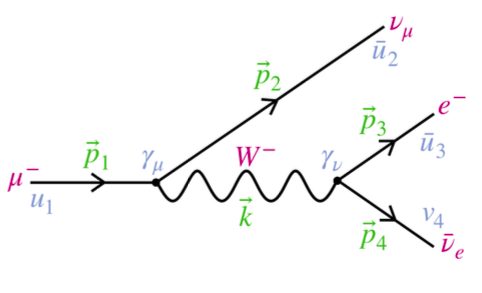
\includegraphics[width=0.55\textwidth]{Figure/5-SM/decadimento muone.png}
    \caption{Processo di decadimento del muone.}
    \label{fig:5 decadimento muone}
\end{figure}

Abbiamo:
\begin{equation}
    \mathcal{A} = \frac{(ie)^2}{8\, \sin^2\theta_w}\, \bra{\psi_\mu}\overline{\psi}_\mu\, \gamma^\rho\, (1-\gamma_5)\, W_\rho^-\, \psi_{\nu_\mu}\cdot\overline{\psi}_{\nu_e}\, \gamma^\sigma\, (1-\gamma_5)\, W_\sigma^+\, \psi_e\, \ket{\overline{\psi}_{\nu_\mu}\, \overline{\psi}_e\, \psi_{\nu_e}}
\end{equation}
così che:
\begin{align}
    M &= \frac{(ie)^2}{8\, \sin^2\theta_w}\, \overline{u}_2\, \gamma^\rho\, (1-\gamma_5)\, u_1\, \frac{(-i\eta_{\rho\sigma})}{s-M_w^2}\, \overline{u}_3\, \gamma^\sigma\, (1-\gamma_5)\, \nu_4 \\
    &= \frac{ie^2}{8\, \sin^2\theta_w\, (s-M_w^2)}\, \overline{u}_2\, \gamma^\rho\, (1-\gamma_5)\, u_1\cdot\overline{u}_3\, \gamma_\rho\, (1-\gamma_5)\, \nu_4
\end{align}
e di conseguenza:
\begin{align}
    |\mathcal{M}|^2 &= \frac{e^4}{2^7\, \sin^4\theta_w\, (s-M_w^2)^2}\sum_{spin}\Big( \overline{u}_2\, \gamma^\rho\, (1-\gamma_5)\, u_1 \Big)\, \Big( \overline{u}_3\, \gamma_\rho\, (1-\gamma_5)\, \nu_4 \Big)\cross \notag \\
    &\qquad \cross \Big( \overline{u}_1\, \gamma^\sigma\, (1-\gamma_5)\, u_2 \Big)\, \Big( \overline{\nu}_4\, \gamma_\sigma\, (1-\gamma_5)\, u_3 \Big) \\
    &= \frac{M_w^4\, G_F^2}{4\, (s-M_w^2)^2}\, \Tr{(\slashed{p}_1 + m_\mu)\, \gamma^\sigma\, (1-\gamma_5)\, (\slashed{p}_2)\, \gamma^\rho\, (1-\gamma_5)}\cross \notag \\
    &\qquad \cross \Tr{(\slashed{p}_3 + m_e)\, \gamma_\rho\, (1-\gamma_5)\, (\slashed{p}_4)\, \gamma_\sigma\, (1-\gamma_5)} \\
    &= \frac{M_w^4\, G_F^2}{(s-M_w^2)^2}\, (p_2)_\beta\, (p_4)^\tau\, \Tr{(\slashed{p}_1 + m_\mu)\, \gamma^\sigma\, \gamma^\beta\, \gamma^\rho\, (1-\gamma_5)}\cross \notag \\
    &\qquad \cross \Tr{(\slashed{p}_3 + m_e)\, \gamma_\rho\, \gamma_\tau\, \gamma_\sigma\, (1-\gamma_5)} \\
    &= \frac{M_w^4\, G_F^2}{(s-M_w^2)^2}\, (p_1)_\alpha\, (p_2)_\beta\, (p_3)^\epsilon\, (p_4)^\tau\, \Tr{\gamma^\alpha\, \gamma^\sigma\, \gamma^\beta\, \gamma^\rho\, (1-\gamma_5)}\, \cross \notag \\
    &\qquad \cross \Tr{\gamma_\epsilon\, \gamma_\rho\, \gamma_\tau\, \gamma_\sigma\, (1-\gamma_5)} \\
    &= \frac{2^4\, M_w^4\, G_F^2}{(s-M_w^2)^2}\, (p_1)_\alpha\, (p_2)_\beta\, (p_3)^\epsilon\, (p_4)^\tau\, \Big[ \eta^{\alpha\sigma}\, \eta^{\beta\rho} + \eta^{\alpha\rho}\, \eta^{\beta\sigma} - \eta^{\alpha\beta}\, \eta^{\sigma\rho} - i\varepsilon^{\alpha\sigma\beta\rho} \Big] \cross \notag \\
    &\qquad \cross \Big[ \eta_{\epsilon\sigma}\, \eta_{\tau\rho} + \eta_{\epsilon\rho}\, \eta^{\tau\sigma} - \eta_{\epsilon\tau}\, \eta_{\sigma\rho} - i\varepsilon_{\epsilon\rho\tau\sigma} \Big] \\
    &= \frac{2^4\, M_w^4\, G_F^2}{(s-M_w^2)^2}\, (p_1)_\alpha\, (p_2)_\beta\, (p_3)^\epsilon\, (p_4)^\tau\, \Big[ \left( \eta^{\alpha\sigma}\, \eta^{\beta\rho} + \eta^{\alpha\rho}\, \eta^{\beta\sigma} - \eta^{\alpha\beta}\, \eta^{\sigma\rho} \right)\, \cross \notag \\
    &\qquad \cross \left( \eta_{\epsilon\sigma}\, \eta_{\tau\rho} + \eta_{\epsilon\rho}\, \eta^{\tau\sigma} - \eta_{\epsilon\tau}\, \eta_{\sigma\rho} \right) - \varepsilon^{\alpha\sigma\beta\rho}\, \varepsilon_{\epsilon\rho\tau\sigma} \Big] \\
    &= \frac{2^4\, M_w^4\, G_F^2}{(s-M_w^2)^2}\, (p_1)_\alpha\, (p_2)_\beta\, (p_3)^\epsilon\, (p_4)^\tau\, \Big[ 2\, \left( \delta_\epsilon^\alpha\, \delta_\tau^\beta + \delta_\tau^\alpha\, \delta_\epsilon^\beta \right) - \notag \\
    &\qquad - 2\, \left( \delta_\epsilon^\alpha\, \delta_\tau^\beta - \delta_\tau^\alpha\, \delta_\epsilon^\beta \right) \Big] \\
    &= \frac{2^4\, M_w^4\, G_F^2}{(s-M_w^2)^2}\, 4\, (p_1\cdot p_4)\, (p_2\cdot p_3) \\
    &= \frac{2^4\, M_w^4\, G_F^2}{(s-M_w^2)^2}\, t^2.
\end{align}


\subsection{Bosoni fisici e costanti di accoppiamento}

Per comodità possiamo definire:
\begin{align}
    W_\mu &= W_\mu^a\, \sigma^a \\
    &= \begin{pmatrix}
        W^3_\mu & W_\mu^1 - i\, W_\mu^2 \\
        W_\mu^1 + iW_\mu^2 & -W_\mu^3
    \end{pmatrix} \\
    &= \begin{pmatrix}
        W_\mu^3 & \sqrt{2}\, W_\mu^\dagger \\
        \sqrt{2}\, W_\mu^- & - W_\mu^3
    \end{pmatrix}
\end{align}
in cui abbiamo posto:
\begin{equation}
    W_\mu^\pm = \frac{W_\mu^1 \mp iW_\mu^2}{\sqrt{2}}
\end{equation}
e quindi usiamo:
\begin{equation}
    \sigma_\pm = \frac{1}{2}\, (\sigma_1 \pm i\sigma_2)
\end{equation}
dunque:
\begin{align}
    W_\mu^+\, \sigma_+ + W_\mu^-\, \sigma_- &= \frac{1}{2\sqrt{2}}\, \Big[ (\sigma_1 + i\sigma_2)\, (W_\mu^1 - iW_\mu^2) + (\sigma_1 - i\sigma_2)\, (W_\mu^1 + iW_\mu^2) \Big] \\
    &= \frac{1}{\sqrt{2}}\, (W_\mu^1\, \sigma_1 + W_\mu^2\, \sigma_2).
\end{align}
Sappiamo che $SU(2) \cross SU(1)$ descrive la corrente elettro-debole, che è composta da una corrente debole carica, una debole neutra e la corrente elettromagnetica.

Possiamo usare $W_\mu^\pm$ per mediare la corrente debole carica e vogliamo utilizzare una combinazione lineare dei due bosoni rimanenti per mediare la corrente debole neutra e l'elettromagnetismo, per ciò introduciamo una matrice di rotazione $R$ ortogonale ($R^T R = \mathbb{1}$):
\begin{align}
    &\begin{pmatrix}
        A_\mu \\
        Z_\mu
    \end{pmatrix} = \begin{pmatrix}
        \cos\theta_w & \sin\theta_w \\
        -\sin\theta_w & \cos\theta_w
    \end{pmatrix}\, \begin{pmatrix}
        B_\mu \\
        W_\mu^3
    \end{pmatrix} \\
    &\begin{cases}
        A_\mu = \sin\theta_w\, W_\mu^3 + \cos\theta_w\, B_\mu \\
        Z_\mu = \cos\theta_w\, W_\mu^3 - \sin\theta_w\, B_\mu
    \end{cases}
\end{align}
che invertendo abbiamo:
\begin{align}
    &\begin{pmatrix}
        W_\mu^3 \\
        B_\mu
    \end{pmatrix} = \begin{pmatrix}
        \cos\theta_w & \sin\theta_w \\
        -\sin\theta_w & \cos\theta_w
    \end{pmatrix}\, \begin{pmatrix}
        Z_\mu \\
        A_\mu
    \end{pmatrix} \\
    &\begin{cases}
        B_\mu = \cos\theta_w\, A_\mu - \sin\theta_w\, Z_\mu \\
        W_\mu^3 = \sin\theta_w\, A_\mu + \cos\theta_w\, Z_\mu
    \end{cases}
\end{align}
nota che vale $\theta_w\approx 28\unit{\degree}$, detto \textit{angolo di Weinberg}, oppure angolo di weak mixing. Questa scelta per $Z$ e $A$ è giustificata anche dal fatto che nella rottura di simmetria tramite Higgs la combinazione che forma $Z$ acquisisce massa, mentre $A$ rimane massless.

Dafiniamo la derivata covariante come:
\begin{equation}
    D_\mu = \partial_\mu + ig_1\, \frac{Y}{2}\, B_\mu + \frac{i}{2}\, g_2\, W_\mu^a\, \sigma^a
\end{equation}
in cui il primo fattore $1/2$ è una convenzione, mentre il secondo è dovuto al fatto che il generatore di $SU(2)$ sia $T^a = \sigma^a\, 1/2$. Questa scelta di derivata covariante rende la lagrangiana invariante rispetto a trasformazioni locali di $SU(2) \cross U(1)$, inoltre bisogna ricordare che quando applichiamo questa derivata covariante un un singoletto di $SU(2)$, il termine con $W$ è nullo.

Le costanti di accoppiamento verranno fissate imponendo la carica elettrica di elettrone e neutrino Left, tramite lo studio della derivata covariante per il doppietto Left:
\begin{align}
    D_\mu L &= \partial_\mu L + ig_1\, \frac{Y}{2}\, B_\mu\, \begin{pmatrix}
        \nu_L \\
        l_L
    \end{pmatrix} + \frac{i}{2}\, g_2\, \begin{pmatrix}
        W_\mu^3 & \sqrt{2}\, W_\mu^+ \\
        \sqrt{2}\, W_\mu^- & -W_\mu^3
    \end{pmatrix}\, \begin{pmatrix}
        \nu_L \\
        l_L
    \end{pmatrix} \\
    &= \partial_\mu L + \frac{i}{2}\, \begin{pmatrix}
        g_1\, Y\, B_\mu + g_2\, W_\mu^3 & \sqrt{2}\, g_2\, W_\mu^+ \\
        \sqrt{2}\, g_2\, W_\mu^- & g_1\, Y\, B_\mu - g_2\, W_\mu^3
    \end{pmatrix}\, \begin{pmatrix}
        \nu_L \\
        l_L
    \end{pmatrix} \\
    &= \partial_\mu L + \frac{i}{2}\, \begin{pmatrix}
        \left(g_1\, Y\, B_\mu + g_2\, W_\mu^3\right)\, \nu_L + \left(\sqrt{2}\, g_2\, W_\mu^+\right)\, l_L \\
        \left(g_1\, Y\, B_\mu - g_2\, W_\mu^3\right)\, l_L + \left(\sqrt{2}\, g_2\, W_\mu^-\right)\, \nu_L
    \end{pmatrix}.
\end{align}
Anche:
\begin{align}
    \overline{L}\, \slashed{D}\, L &= \overline{L}\, \slashed{\partial}\, L + \overline{L}\, \gamma^\mu\, J_\mu^{ew}\, L + \overline{L}\, \gamma^\mu\, J_{\mu}^{cc}\, L \\
    &= \overline{L}\, \slashed{\partial}\, L + \frac{i}{2}\Big[ \overline{\nu}_L\, \gamma^\mu\, \left( g_1\, Y\, B_\mu + g_2\, W_\mu^3 \right)\, \nu_L + \overline{l}_L\, \gamma^\mu\, \left( g_1\, Y\, B_\mu - g_2\, W_\mu^3 \right)\, l_L \Big] + \notag \\
    &\qquad + \frac{i}{2}\, \sqrt{2}\, g_2\, \Big( \overline{\nu}_L\, \gamma^\mu\, W_\mu^+\, l_L + \overline{l}_L\, \gamma^\mu\, W_\mu^-\, \nu_L \Big).
\end{align}
Studiamo la corrente elettrodebole:
\begin{align}
    \overline{L}\, \gamma^\mu\, J_\mu^{ew}\, L &= \frac{i}{2}\, \Bigg[ \overline{\nu}_L\, \gamma^\mu\Big( g_1\, Y\, B_\mu + g_2\, W_\mu^3 \Big)\, \nu_L + \overline{l}_L\, \gamma^\mu\Big( g_1\, Y\, B_\mu - g_2\, W_\mu^3 \Big)\, l_L \Bigg] \\
    &= \frac{i}{2}\, \overline{\nu}_L\, \gamma^\mu\Bigg[ \left( g_1\, Y\, \cos\theta_w + g_2\, \sin\theta_w \right)\, A_\mu - \left( g_1\, Y\, \sin\theta_w - g_2\, \cos\theta_w \right)\, Z_\mu \Bigg]\, \nu_L + \notag \\
    &\qquad + \frac{i}{2}\, \overline{l}_L\, \gamma^\mu\Bigg[ \left( g_1\, Y\, \cos\theta_w - g_2\, \sin\theta_w \right)\, A_\mu - \left( g_1\, Y\, \sin\theta_w + g_2\, \cos\theta_w \right)\, Z_\mu \Bigg]\, l_L
\end{align}
siccome $A$ media la corrente elettromagnetica, quindi dobbiamo imporre la carica elettrica:
\begin{equation}
    \begin{cases}
        \nu_L\ :\quad \frac{1}{2}\Big( g_1\, Y\, \cos\theta_w + g_2\, \sin\theta_w \Big) = 0 \\
        l_L\ :\quad \frac{1}{2}\Big( g_1\, Y\, \cos\theta_w - g_2\, \sin\theta_w \Big) = e \\
    \end{cases}
\end{equation}
ovvero:
\begin{equation}
    -g_2\, \sin\theta_w = g_1\, Y\, \cos\theta_w = e
\end{equation}
se imponiamo che l'ipercarica del doppietto Left sia $Y(L)=-1$, allora:
\begin{equation}
    g_2\, \sin\theta_w = g_1\, \cos\theta_w = - e
\end{equation}
ovvero:
\begin{equation}
    g_1 = -\frac{e}{\cos\theta_w}\quad , \quad g_2 = -\frac{e}{\sin\theta_w}
\end{equation}
che se sostituite nella corrente elettrodebole:
\begin{align}
    \overline{L}\, \gamma^\mu\, J_\mu^{ew}\, L &= ie\, \overline{l}_L\, \gamma^\mu\, A_\mu\, l_L - \frac{i}{2}\, \Bigg[ \overline{\nu}_L\, \gamma^\mu\, \left( g_1\, Y\, \sin\theta_w - g_2\, \cos\theta_w \right)\, \nu_L + \notag \\
    &\qquad + \overline{l}_L\, \gamma^\mu\, \left( g_1\, Y\, \sin\theta_w + g_2\, \cos\theta_w \right)\, l_L \Bigg]\, Z_\mu \\
    &= ie\, \overline{l}_L\, \gamma^\mu\, A_\mu\, l_L + \frac{i\, e}{2\sin\theta_w\, \cos\theta_w}\, \Bigg[ -\overline{\nu}_L\, \gamma^\mu\, \Big( \sin^2\theta_w + \cos^2\theta_w \Big)\, \nu_L + \notag \\
    &\qquad + \overline{l}_L\, \gamma^\mu\, \Big( \sin^2\theta_w - \cos^2\theta_w \Big)\, l_L \Bigg]\, Z_\mu \\
    &= -i\, e\Bigg[ -\overline{l}_L\, (\gamma^\mu\, A_\mu)\, l_L + \frac{1}{\sin{(2\theta_w)}}\, \overline{\nu}_L\, (\gamma^\mu\, Z_\mu)\, \nu_L - \notag \\
    &\qquad - \frac{1}{\tan{(2\theta_w)}}\, \overline{l}_L\, (\gamma^\mu\, Z_\mu)\, l_L \Bigg].
\end{align}


\subsection{Numeri quantici e campi}

Possiamo riscrivere la matrice di Pauli in funzione dell'isospin:
\begin{equation}
    I_3 = \frac{1}{2}\, \sigma_3
\end{equation}
e ciò ci permette di ricavare la formula di Gell-Mann e Nishijima:
\begin{equation}
    Q = \frac{Y}{2} + I_3
\end{equation}
che usiamo per ricavare l'ipercarica ($Y$) che è uguale per tutti i membri dello stesso multipletto. Ricordiamo che per i singoletti l'isospin vale $I_3 = 0$, mentre per i doppietti è:
\begin{equation}
    I_3 = +\frac{1}{2}
\end{equation}
per la prima componente e:
\begin{equation}
    I_3 = -\frac{1}{2}
\end{equation}
per la seconda. Abbiamo:
\begin{equation}
    L = \begin{pmatrix}
        \nu_L \\
        l_L
    \end{pmatrix}
\end{equation}
è un doppietto rispetto a $SU(2)$ ed è carico rispetto ad $U(1)$; $l_R$ è un singoletto rispetto ad $SU(2)$ ($I_3=0$) ed è carico rispetto ad $U(1)$. Il campo di Higgs è un doppietto di $SU(2)$ ed è carico rispetto ad $U(1)$, pertanto lo definiamo come:
\begin{equation}
    \Phi = \begin{pmatrix}
        \phi^+ \\
        \phi^0
    \end{pmatrix}
\end{equation}
dove $\phi^+$, $\phi^0$ sono due campi complessi e $\phi^+$ ha carica $+1$. \\

Riassumiamo il tutto nella tabella \ref{tab:5 riassunto numeri quantici SM}.
\begin{figure}[ht!]
    \centering
\begin{tabular}{|c|c|c|c|c|c|c|c|c|c|c|}
        \hline
        \rule{0pt}{3ex}
         & \multicolumn{2}{|c|}{Higgs} & \multicolumn{4}{|c|}{Leptoni} & \multicolumn{4}{|c|}{Quarks} \\[1ex]
        \hline
        \rule{0pt}{3ex}
         & $\phi^+$ & $\phi^0$ & $\nu_L$ & $l_L$ & $\nu_R$ & $l_R$ & $u_L$ & $d_L$ & $u_R$ & $d_R$ \\[1ex]
        \hline
        \rule{0pt}{3ex}
        $Q$ & +1 & 0 & 0 & -1 & 0 & -1 & $+\frac{2}{3}$ & $-\frac{1}{3}$ & $+\frac{2}{3}$ & $-\frac{1}{3}$ \\[1ex]
        \hline
        \rule{0pt}{3ex}
        $I_3$ & $+\frac{1}{2}$ & $-\frac{1}{2}$ & $+\frac{1}{2}$ & $-\frac{1}{2}$ & 0 & 0 & $+\frac{1}{2}$ & $-\frac{1}{2}$ & 0 & 0 \\[1ex]
        \hline
        \rule{0pt}{3ex}
        $Y$ & $+1$ & $+1$ & $-1$ & $-1$ & 0 & -2 & $+\frac{1}{3}$ & $+\frac{1}{3}$ & $+\frac{4}{3}$ & $-\frac{2}{3}$ \\[1ex]
        \hline
    \end{tabular}
    \caption{}
    \label{tab:5 riassunto numeri quantici SM}
\end{figure}


\subsection{Lagrangiana massless dei leptoni}

Riassumendo, per il doppietto Left abbiamo:
\begin{equation}
    \overline{L}\slashed{D} L = \overline{L}\, \slashed{\partial}\, L + \overline{L}\, \gamma^\mu\, J_\mu^{ew}\, L + \overline{L}\, \gamma^\mu\, J_{\mu}^{cc}\, L
\end{equation}
in cui:
\begin{align}
    &\overline{L}\, \gamma^\mu\, J_\mu^{ew}\, L = -i\, e\Bigg[ -\overline{l}_L\, (\gamma^\mu\, A_\mu)\, l_L + \frac{1}{\sin{(2\theta_w)}}\, \overline{\nu}_L\, (\gamma^\mu\, Z_\mu)\, \nu_L - \frac{1}{\tan{(2\theta_w)}}\, \overline{l}_L\, (\gamma^\mu\, Z_\mu)\, l_L \Bigg] \\
    &\overline{L}\, \gamma^\mu\, J_\mu^{cc}\, L = -\frac{i\, e}{\sqrt{2}\, \sin\theta_w}\, \Big( \overline{\nu}_L\, \gamma^\mu\, W_\mu^+\, l_L + \overline{l}_L\, \gamma^\mu\, W_\mu^-\, \nu_L \Big)
\end{align}
mentre per i singoletti Right abbiamo:
\begin{equation}
    \overline{l}_R\, \slashed{D} l_R = \overline{l}_R\, \slashed{\partial}\, l_R + i\, e\, \overline{l}_R\, \gamma^\mu\, \Big( A_\mu - \tan\theta_w\, Z_\mu \Big)\, l_R
\end{equation}
il neutrino Right è completamente disaccoppiato, nel senso che non abbiamo interazioni elettrodeboli.

Infine osserviamo che nei termini puramente cinetici la parte L e quella la R sono identiche, quindi possiamo scriverli come:
\begin{equation}
    \overline{l}_L\, \slashed{\partial}\, l_L + \overline{\nu}_L\, \slashed{\partial}\, \nu_L + \overline{l}_R\, \slashed{\partial}\, l_R + \overline{\nu}_R\, \slashed{\partial}\, \nu_R = \overline{l}\, \slashed{\partial}\, l + \overline{\nu}\, \slashed{\partial}\, \nu.
\end{equation}
Possiamo scrivere la lagrangiana del settore leptonico come:
\begin{align}
    \Lag_{lep} &= i\overline{L}\, \slashed{D}\, L + i\overline{l}_R\, \slashed{D}\, l_R + i\overline{\nu}_R\, \slashed{D}\, \nu_R \\
    &= i\overline{l}\, \slashed{\partial}\, l + i\overline{\nu}\, \slashed{\partial}\nu - e\, \left(\overline{l}\, \gamma^\mu\, l\right)\, A_\mu + e\, \Bigg[ \frac{1}{\sin{(2\theta_w)}}\, \overline{\nu}_L\, \gamma^\mu\, \nu_L - \notag \\
    &\qquad - \frac{1}{\tan{(2\theta_w)}}\, \overline{l}_L\, \gamma^\mu\, l_L + \tan\theta_w\, \overline{l}_R\, \gamma^\mu\, l_R \Bigg]\, Z_\mu + \notag \\
    &\qquad + \frac{e}{\sqrt{2}\, \sin\theta_w}\, \Big( \overline{\nu}_L\, \gamma^\mu\, W_\mu^+\, l_L + \overline{l}_L\, \gamma^\mu\, W_\mu^-\, \nu_L \Big)
\end{align}
in cui il primo termine sono i termini \textit{cinetici e di corrente elettromagnetica}, il secondo la \textit{corrente debole neutra} e l'ultimo la \textit{corrente debole carica}. Osserviamo che le correnti deboli (neutre e cariche) si accoppiano in modo diverso con le componenti left e right, questo è sintomo del fatto che le interazioni deboli violano la parità. \\

Riscriviamo la lagrangiana usando i proiettori Left e Right:
\begin{equation}
    P_L = \frac{1 - \gamma_5}{2} \quad , \quad P_R = \frac{1 + \gamma_5}{2}
\end{equation}
e per entrambi vale $(P_{L,R})^2 = P_{L,R}^\dagger = P_{L,R}$. Osserviamo che:
\begin{align}
    \overline{\psi}_L\, (\gamma^\mu\, B_\mu)\, \phi_L &= \psi^\dagger\, P_L\, \gamma^0\, \gamma^\mu\, B_\mu\, P_L\, \phi \\
    &= \psi^\dagger\, \gamma^0\, \gamma^\mu\, (P_L)^2\, B_\mu\, \phi \\
    &= \overline{\psi}\, \gamma^\mu\, P_L\, B_\mu\, \phi
\end{align}
e analogamente per $R$. Scriviamo:
\begin{align}
    \Lag_{lep} &= i\overline{l}\, \slashed{\partial}\, l + i\overline{\nu}\, \slashed{\partial}\, \nu - e\, \left(\overline{l}\, \gamma^\mu\, l\right)\, A_\mu + \notag \\
    &\qquad + \frac{e}{2\sin{2\theta_w}}\, \Big[ \overline{\nu}\, \gamma^\mu\, (1-\gamma_5)\, \nu + \overline{l}\, \gamma^\mu\, \big( 4\sin^4\theta_w - 1 + \gamma_5 \big)\, l \Big]\, Z_\mu + \notag \\
    &\qquad + \frac{e}{2\sqrt{2}\, \sin\theta_w}\Big( \overline{\nu}\, \gamma^\mu\, (1-\gamma_5)\, W_\mu^+\, l + \overline{l}\, \gamma^\mu\, (1-\gamma_5)\, W_\mu^-\, \nu \Big).
\end{align}

\paragraph{Annotazioni.}Nel studiare il settore leptonico abbiamo un po' barato, nel senso che se teniamo le componenti L/R esplicite non dovremmo utilizzare $\gamma^\mu$ (matrici 4x4) bensì le $\sigma^\mu$ (matrici 2x2) per le componenti R e le $\overline{\sigma}^\mu$ (matrici 2x2) per le componenti L. Ricordiamo che $\sigma^\mu = (\mathbb{1},\vec{\sigma})$ e $\overline{\sigma}^\mu = (\mathbb{1},-\vec{\sigma})$, inoltre in rappresentazione di Weyl abbiamo:
\begin{equation}
    \gamma^\mu = \begin{pmatrix}
        0 & \sigma^\mu \\
        \overline{\sigma}^\mu & 0
    \end{pmatrix}
\end{equation}
e possiamo osservare che:
\begin{equation}
    \gamma^0\, \gamma^\mu = \begin{pmatrix}
        0 & 1 \\
        1 & 0
    \end{pmatrix}\, \begin{pmatrix}
        0 & \sigma^\mu \\
        \overline{\sigma}^\mu & 0
    \end{pmatrix} = \begin{pmatrix}
        \overline{\sigma}^\mu & 0 \\
        0 & \sigma^\mu
    \end{pmatrix}.
\end{equation}
In più, nel nostro disorso abbiamo utilizzato un abuso di notazione per cui:
\begin{equation}
    \psi_L = \begin{pmatrix}
        \psi_L \\
        0
    \end{pmatrix} \quad , \quad \psi_R = \begin{pmatrix}
        0 \\
        \psi_R
    \end{pmatrix}
\end{equation}
questo abuso è compatibile con le relazioni dei proiettori:
\begin{equation}
    \psi_R = \frac{1 + \gamma_5}{2}\, \psi \quad , \quad \psi_L = \frac{1-\gamma_5}{2}\, \psi
\end{equation}
inoltre:
\begin{equation}
    \psi = \psi_R + \psi_L
\end{equation}
che ci giustifica l'uso della $\gamma$. Riarrangiando i termini ritroviamo la lagrangiana:
\begin{align}
    \Lag_K &= L^\dagger\, \overline{\sigma}^\mu\, i\, D_\mu\, L + l_R^\dagger\, \sigma^\mu\, i\, D_\mu\, l_R + \nu_R^\dagger\, \sigma^\mu\, i\, D_\mu\, \nu_R \\
    &= i\Big( l_L^\dagger\, \overline{\sigma}^\mu\, D_\mu\, l_L + l_R^\dagger\, \sigma^\mu\, D_\mu\, l_R \Big) + i\, \Big( \nu_L^\dagger\, \overline{\sigma}^\mu\, D_\mu\, \nu_L + \nu_R^\dagger\, \sigma^\mu\, D_\mu\, \nu_R \Big) \\
    &= \begin{pmatrix}
        l_L^\dagger & l_R^\dagger
    \end{pmatrix} \begin{pmatrix}
        \overline{\sigma}^\mu & 0 \\
        0 & \sigma^\mu
    \end{pmatrix} (iD_\mu) \begin{pmatrix}
        l_L \\
        l_R
    \end{pmatrix} + \begin{pmatrix}
        \nu_L^\dagger & \nu_R^\dagger
    \end{pmatrix} \begin{pmatrix}
        \overline{\sigma}^\mu & 0 \\
        0 & \sigma^\mu
    \end{pmatrix} (iD_\mu) \begin{pmatrix}
        \nu_L \\
        \nu_R
    \end{pmatrix} \\
    &= \begin{pmatrix}
        l_L^\dagger & l_R^\dagger
    \end{pmatrix} \gamma^0 \gamma^\mu (iD_\mu) \begin{pmatrix}
        l_L \\
        l_R
    \end{pmatrix} + \begin{pmatrix}
        \nu_L^\dagger & \nu_R^\dagger
    \end{pmatrix} \gamma^0 \gamma^\mu (iD_\mu) \begin{pmatrix}
        \nu_L \\
        \nu_R
    \end{pmatrix} \\
    &= \overline{l}\, (i\gamma^\mu\, D_\mu)\, l + \overline{\nu}\, (i\gamma^\mu\, D_\mu)\, \nu.
\end{align}





\section{Settore di Higgs}

I riferimenti sono p. 527-530 dello Srednicki \cite{Srednicki}. \\

Per definizione l'Higgs si trasforma in maniera non banale rispetto $SU(2)\cross SU(1)$, come:
\begin{equation}
    \Phi \quad \longrightarrow \quad e^{-i\theta}\, U\, \Phi
\end{equation}
mentre non interagisce con i quark essendo essi doppietti di $SU(3)$. Consideriamo:
\begin{equation}
    \Lag_H = \left(D_\mu\, \Phi\right)^\dagger\, \left(D^\mu\, \Phi\right) - V(\Phi^\dagger\, \Phi)
\end{equation}
che è invariante per trasformazioni locali di $SU(2)\cross SU(1)$ se definiamo la derivata covariante come:
\begin{equation}
    D_\mu = \partial_\mu + ig_1\, \frac{Y}{2}\, B_\mu + \frac{i}{2}\, g_2\, W_\mu^a\, \sigma^a
\end{equation}
dove il primo fattore $1/2$ è una convenzione, mentre il secondo è dovuto al fatto che il generatore di $SU(2)$ è $T^a = \sigma^a\, 1/2$, inoltre abbiamo visto che $Y(\Phi) = +1$. Ricordiamo che abbiamo definito:
\begin{align}
    W_\mu &= W_\mu^a\, \sigma^a \\
    &= \begin{pmatrix}
        W_\mu^3 & W_\mu^1 - iW_\mu^2 \\
        W_\mu^1 + iW_\mu^2 & -W_\mu^3
    \end{pmatrix} \\
    &= \begin{pmatrix}
        W_\mu^3 & \sqrt{2}\, W_\mu^+ \\
        \sqrt{2}\, W_\mu^- & -W_\mu^3
    \end{pmatrix}
\end{align}
in cui avevamo posto:
\begin{equation}
    W_\mu^\pm = \frac{W_\mu^1 \mp iW_\mu^2}{\sqrt{2}}
\end{equation}
ossia utilizziamo $\sigma^\pm$ anziché $\sigma_1$ e $\sigma_2$. Con questa Sostituzione i termini cinetici diventano:
\begin{equation}
    \begin{cases}
        F_{\mu\nu}^1 = \partial_\mu W_\nu^1 - \partial_\nu W_\mu^1 - g_2\, \left( W_\mu^2\, W_\nu^3 - W_\mu^3\, W_\nu^2 \right) \\
        F_{\mu\nu}^2 = \partial_\mu W_\nu^2 - \partial_\nu W_\mu^2 - g_2\, \left( W_\mu^1\, W_\nu^3 - W_\mu^3\, W_\nu^1 \right) \\
        F_{\mu\nu}^3 = \partial_\mu W_\nu^3 - \partial_\nu W_\mu^3 - g_2\, \left( W_\mu^1\, W_\nu^2 - W_\mu^2\, W_\nu^1 \right)
    \end{cases}
\end{equation}
cioè:
\begin{equation}
    \begin{cases}
        F_{\mu\nu}^+ = \partial_\mu W_\nu^+ - \partial_\nu W_\mu^+ - g_2\, \left( W_\mu^3\, W_\nu^- - W_\mu^-\, W_\nu^3 \right) \\
        F_{\mu\nu}^- = \partial_\mu W_\nu^- - \partial_\nu W_\mu^- + g_2\, \left( W_\mu^3\, W_\nu^+ - W_\mu^+\, W_\nu^3 \right) \\
        F_{\mu\nu}^3 = \partial_\mu W_\nu^3 - \partial_\nu W_\mu^3 - g_2\, \left( W_\mu^-\, W_\nu^+ - W_\mu^+\, W_\nu^- \right)
    \end{cases}
\end{equation}
quindi per la parte $SU(2)\cross SU(1)$ (forza elettrodebole di YM) e la parte di Higgs abbiamo:
\begin{equation}
    \Lag_{YMH} = -\frac{1}{4}\, B_{\mu\nu}\, B^{\mu\nu} - \frac{1}{4}\, F_{\mu\nu}^3\, F^{3,\mu\nu} - \frac{1}{2}\, F_{\mu\nu}^+\, F^{-,\mu\nu} + \left(D^\mu\Phi\right)^\dagger\, \left(D_\mu\Phi\right) - V(\Phi^\dagger\, \Phi).
\end{equation}


\subsection{Rottura della simmetria tramite Higgs}

Possiamo scegliere:
\begin{equation}
    V(\Phi^\dagger\, \Phi) = \frac{m^2}{2\, \phi_0^2}\, \left( \Phi^\dagger\, \Phi - \phi_0^2 \right)^2 \geq 0
\end{equation}
la scelta di questo potenziale fa sì che tutta la lagrangiana sia invariante rispetto a $SU(2) \cross SU(1)$ locali. Vogliamo studiare il vuoto di questa teoria, siccome il potenziale è definito positivo abbiamo che il minimo del potenziale si trova per:
\begin{equation}
    \Phi^\dagger\, \Phi - \phi_0^2 = |\Phi_A|^2 + |\Phi_B|^2 - \phi_0^2 = 0
\end{equation}
una delle soluzioni (quella che si prende convenzionalmente) è:
\begin{equation}
    \langle\Phi_A\rangle = 0 \quad , \quad \langle\Phi_B\rangle = \phi_0
\end{equation}
ovvero la configurazione di vuoto è:
\begin{equation}
    \langle\Phi\rangle = \begin{pmatrix}
        0 \\
        \phi_0
    \end{pmatrix}
\end{equation}
e siccome $\phi_0\neq 0$ rispetta le simmetrie di Poincarè. Possiamo espandere rispetto al vuoto considerando $\Phi = \langle\Phi\rangle + \phi$, in cui:
\begin{equation}
    \phi = \begin{pmatrix}
        \phi_A \\
        \phi_B
    \end{pmatrix}
\end{equation}
sono le oscillazioni di vuoto e ha 4 gradi di libertà (2 per ogni componente). \\

Vogliamo anche verificare quali simmetrie sono preservate dal vuoto. Per $\sigma^\pm$ abbiamo:
\begin{equation}
    \begin{pmatrix}
        0 & X \\
        Y & 0
    \end{pmatrix}\begin{pmatrix}
        0 \\
        \phi_0
    \end{pmatrix} \neq \begin{pmatrix}
        0 \\
        \phi_0
    \end{pmatrix}
\end{equation}
cioè il vuoto rompe spontaneamente i generatori $\sigma^1$ e $\sigma^2$ di $SU(2)$, analogamente per $\sigma^3$ abbiamo:
\begin{equation}
    \begin{pmatrix}
        X & 0 \\
        0 & -X
    \end{pmatrix}\begin{pmatrix}
        0 \\
        \phi_0
    \end{pmatrix} \neq \begin{pmatrix}
        0 \\
        \phi_0
    \end{pmatrix}
\end{equation}
e per $U(1)$ abbiamo:
\begin{equation}
    e^{-i\theta}\, \begin{pmatrix}
        0 \\
        \phi_0
    \end{pmatrix} \neq \begin{pmatrix}
        0 \\
        \phi_0
    \end{pmatrix} \qquad , \quad \forall\theta\neq 0.
\end{equation}
Quindi apparentemente il vuoto rompe tutti i generatori, tuttavia se combiniamo le due trasformazioni $\sigma^3$ e $U(1)$, abbiamo che:
\begin{align}
    e^{-i\theta}\, U\, \Phi &= \begin{pmatrix}
        \exp{-i\left(\theta - \frac{1}{2}\epsilon^3\right)} & 0 \\
        0 & \exp{-i\left(\theta + \frac{1}{2}\epsilon^3\right)}
    \end{pmatrix}\begin{pmatrix}
        0 \\
        \phi_0
    \end{pmatrix} \\
    &= \begin{pmatrix}
        0 \\
        \exp{-i\left(\theta + \frac{1}{2}\epsilon^3\right)}\, \phi_0
    \end{pmatrix}
\end{align}
questa trasformazione lascia il vuoto invariato nel caso in cui $\theta = -\frac{1}{2}\, \epsilon^3$. Quindi dei 4 generatori soltanto uno preserva il vuoto, pertanto abbiamo 3 bosoni di Goldstone che possono essere riassorbiti nei bosoni di gauge e quindi abbiamo 3 bosoni massivi: $W_\mu^\pm$ e un'unica combinazione di $W_\mu^3$ e $B_\mu$ che chiameremo $Z_\mu$ (combinazione ortogonale alla scelta $\theta = -1/2\, \epsilon^3$), infine abbiamo la particella mass-less che preserva il vuoto e rappresenta l'elettromagnetismo ($A_\mu$).


\subsection{Calcolo del potenziale}

Ci possiamo porrè nel gauge unitario dove mettiamo i bosoni di Goldstone a zero perché li possiamo riassorbire tramite una trasformazione di gauge, quindi:
\begin{equation}
    \Phi = \langle\Phi\rangle + \phi = \begin{pmatrix}
        0 \\
        \phi_0 + \frac{h}{\sqrt{2}}
    \end{pmatrix}
\end{equation}
in cui $h$ è il campo scalare reale di Higgs (già correttamente normalizzato). Abbiamo:
\begin{align}
    \Phi^\dagger\, \Phi &= \left(\phi_0 + \frac{h}{\sqrt{2}}\right)^2 \\
    &= \phi_0^2 + \sqrt{2}\, \phi_0\, h + \frac{1}{2}\, h^2 \\
    &= \phi_0^2 + \sqrt{2}\, \phi_0\, \left( 1 + \frac{h}{2\sqrt{2}\, \phi_0} \right)\, h
\end{align}
e anche:
\begin{align}
    V &= \frac{m^2}{2\, \phi_0^2}\, \left( \Phi^\dagger\, \Phi - \phi_0^2\right)^2 \\
    &= m^2\, h^2\, \left( 1 + \frac{h}{2\sqrt{2}\, \phi_0} \right)^2 \\
    &= m^2\, h^2 + \frac{m^2\, h^3}{\sqrt{2}\, \phi_0} + \frac{m^2\, h^4}{8\, \phi_0^2}
\end{align}
quindi la massa di Higgs è $m_h^2 = 2m^2$ e possiamo osservare che aha interazioni $h^3$ e $h^4$, dunque possiamo avere un vertice con 3 o 4 gambe esterne.


\subsection{Calcolo della derivata covariante}

Per calcolare il termine cinetico studiamo la derivata covariante. Per semplicità poniamo:
\begin{equation}
    \eta = \frac{h}{\sqrt{2}}
\end{equation}
e possiamo vedere:
\begin{align}
    D_\mu\, \Phi &= \left[ \partial_\mu + \frac{i}{2}\, g_1\, B_\mu + \frac{i}{2}\, g_2\, \begin{pmatrix}
        W_\mu^3 & \sqrt{2}\, W_\mu^+ \\
        \sqrt{2}\, W_\mu^- & -W_\mu^3
    \end{pmatrix} \right] \begin{pmatrix}
        0 \\
        \phi_0 + \eta
    \end{pmatrix} \\
    &= \begin{pmatrix}
        0 \\
        \partial_\mu\eta
    \end{pmatrix} + \frac{i}{2}\begin{pmatrix}
        g_1\, B_\mu + g_2\, W_\mu^3 & \sqrt{2}\, g_2\, W_\mu^+ \\
        \sqrt{2}\, g_2\, W_\mu^- & g_1\, B_\mu - g_2\, W_\mu^3
    \end{pmatrix}\begin{pmatrix}
        0 \\
        1
    \end{pmatrix}\, \left(\phi_0 + \eta\right) \\
    &= \begin{pmatrix}
        0 \\
        \partial_\mu\eta
    \end{pmatrix} + \frac{i}{2}\begin{pmatrix}
        \sqrt{2}\, g_2\, W_\mu^+ \\
        g_1\, B_\mu - g_2\, W_\mu^3
    \end{pmatrix}\, \left(\phi_0 + \eta\right) \\
    &= \begin{pmatrix}
        \frac{i}{\sqrt{2}}\, g_2\, \left(\phi_0 + \eta\right)\, W_\mu^+ \\
        \partial_\mu\eta + \frac{i}{2}\, \left(\phi_0 + \eta\right)\, \left(g_1\, B_\mu - g_2\, W_\mu^3\right)
    \end{pmatrix}
\end{align}
insieme a:
\begin{equation}
    \left(D_\mu\Phi\right)^\dagger = \Bigg(
        -\frac{i}{\sqrt{2}}\, g_2\, \left(\phi_0 + \eta\right)\, W_\mu^- \quad , \quad \partial_\mu\eta - \frac{i}{2}\, \left(\phi_0 + \eta\right)\, \left(g_1\, B_\mu - g_2\, W_\mu^3\right) \Bigg)
\end{equation}
conseguentemente:
\begin{align}
    \left(D_\mu\Phi\right)^\dagger\, \left(D^\mu\Phi\right) &= \frac{1}{2}\, \partial_\mu h\, \partial^\mu h + \frac{1}{4}\left(\phi_0 + \frac{h}{\sqrt{2}}\right)^2\, \Big[ 2g_2^2\, W_\mu^+\, W^{-,\mu} + \notag \\
    &\qquad + \left( g_1\, B_\mu - g_2\, W_\mu^3 \right)^2 \Big] \\
    &= \frac{1}{2}\, \partial_\mu h\, \partial^\mu h + \frac{1}{4}\left(\phi_0 + \frac{h}{\sqrt{2}}\right)^2\, \Big[ 2g_2^2\, W_\mu^+\, W^{-,\mu} + \notag \\
    &\qquad + \left( g_1^2 + g_2^2 \right)\, Z_\mu\, Z^\mu \Big]
\end{align}
con:
\begin{equation}
    Z_\mu = \frac{g_1\, B_\mu - g_2\, W_\mu^3}{\sqrt{g_1^2 + g_2^2}}.
\end{equation}


\subsection{Lagrangiana di Higgs e masse dei bosoni vettori}

Abbiamo:
\begin{align}
    \Lag_H &= \left(D_\mu\Phi\right)^\dagger\, \left(D^\mu\Phi\right) - V(\Phi^\dagger\, \Phi) \\
    &= \frac{1}{2}\, \partial_\mu h\, \partial^\mu h + \frac{1}{4}\left(\phi_0 + \frac{h}{\sqrt{2}}\right)^2\, \Big[ 2g_2^2\, W_\mu^+\, W^{-,\mu} + \left( g_1^2 + g_2^2 \right)\, Z_\mu\, Z^\mu \Big] - \notag \\
    &\qquad - m^2 h^2 - \frac{m^2\, h^3}{\sqrt{2}\, \phi_0} - \frac{m^2\, h^4}{8\, \phi_0^2} \\
    &= \frac{1}{2}\, \partial_\mu h\, \partial^\mu h - \frac{1}{2}\, m_h^2\, h^2 + \frac{1}{2}\, m_Z^2\, Z_\mu\, Z^\mu + m_W^2\, W_\mu^+\, W^{-,\mu} - \notag \\
    &\qquad - \frac{1}{4}\left(\frac{h^2}{2} + \sqrt{2}\, \phi_0\, h\right)\, \Big[ 2g_2^2\, W_\mu^+\, W^{-,\mu} + \left( g_1^2 + g_2^2 \right)\, Z_\mu\, Z^\mu \Big] - \notag \\
    &\qquad - \frac{m^2\, h^3}{\sqrt{2}\, \phi_0} - \frac{m^2\, h^4}{8\, \phi_0^2} \label{eqn:5 lag Higgs e masse bos vettori}
\end{align}
in cui la prima riga di (\ref{eqn:5 lag Higgs e masse bos vettori}) sono il termine cinetico per $h$ e la masse dei bosoni, mentre la seconda e terza riga rappresentano le interazioni. Le masse dei bosoni di gauge sono:
\begin{equation}
    m_H^2 = 2m^2 \quad , \quad m_W^2 = \frac{\phi_0^2\, g_2^2}{2} \quad , \quad m_Z^2 = \frac{\phi_0^2}{2}\, \left(g_1^2 + g_2^2\right)
\end{equation}
e se sostituiamo:
\begin{equation}
    g_1 = -\frac{e}{\cos\theta_w} \quad , \quad g_2 = -\frac{e}{\sin\theta_w}
\end{equation}
otteniamo:
\begin{equation}
    m_W^2 = \frac{e^2\, \phi_0^2}{2\, \cos^2\theta_w} \quad , \quad m_Z^2 = \frac{e^2\, \phi_0^2}{2}.
\end{equation}


\section{Lagrangiana di Yang-Mills-Higgs}

Possiamo riscrivere:
\begin{equation}
    \sin\theta_w = \frac{g_1}{\sqrt{g_1^2 + g_2^2}} \quad , \quad \cos\theta_w = \frac{g_2}{\sqrt{g_1^2 + g_2^2}}
\end{equation}
in cui $\theta_w$ è detto \textit{angolo di Weinberg}. Dunque abbiamo:
\begin{equation}
    \begin{cases}
        A_\mu = \sin\theta_w\, W_\mu^3 + \cos\theta_w\, B_\mu \\
        Z_\mu = \cos\theta_w\, W_\mu^3 - \sin\theta_w\, B_\mu
    \end{cases}
\end{equation}
ovvero:
\begin{equation}
    \begin{cases}
        B_\mu = \cos\theta_w\, A_\mu - \sin\theta_w\, Z_\mu \\
        W_\mu^3 = \sin\theta_w\, A_\mu + \cos\theta_w\, Z_\mu
    \end{cases}
\end{equation}
in cui $Z$ media la corrente debole neutra e $A$ media l'interazione elettromagnetica. Definiamo inoltre:
\begin{equation}
    \begin{cases}
        A_{\mu\nu} = \partial_\mu A_\nu - \partial_\nu A_\mu \\
        Z_{\mu\nu} = \partial_\mu Z_\nu - \partial_\nu Z_\mu \\
        W_{\mu\nu}^\pm = \partial_\mu W_\nu^\pm - \partial_\nu W_\mu^\pm
    \end{cases}
\end{equation}
che sostituiamo nei termini cinetici di Yang-Mills. Abbiamo:
\begin{align}
    &F_{\mu\nu}^\pm = W_{\mu\nu}^\pm \mp ig_2\, \Big[ \sin\theta_w\, \left(A_\mu W_\nu^\mp - W_\mu^\mp A_\nu \right) + \cos\theta_w\, \left(Z_\mu W_\nu^\mp - W_\mu^\mp Z_\nu \right) \Big] \\
    &F_{\mu\nu}^3 = \Big[ \sin\theta_w\, A_{\mu\nu} + \cos\theta_w\, Z_{\mu\nu} \Big] - ig_2\, \left( W_\mu^-\, W_\nu^+ - W_\mu^+\, W_\nu^- \right) \\
    &B_{\mu\nu} = \partial_\mu B_\nu - \partial_\nu B_\mu = \cos\theta_w\, A_{\mu\nu} - \sin\theta_w\, Z_{\mu\nu}.
\end{align}
Sostituendo otteniamo la lagrangiana che descrive i bosoni di gauge ed Higgs:
\begin{align}
    \Lag_{YMH} &= -\frac{1}{4}\, B_{\mu\nu}\, B^{\mu\nu} - \frac{1}{4}\, F_{\mu\nu}^3\, F^{3,\mu\nu} - \frac{1}{2}\, F_{\mu\nu}^+\, F^{-,\mu\nu} + \left(D^\mu\Phi\right)^\dagger\, \left(D_\mu\Phi\right) - V(\Phi^\dagger\, \Phi) \\
    &= -\frac{1}{4}\, F_{\mu\nu}\, F^{\mu\nu} - \frac{1}{4}\, Z_{\mu\nu}\, Z^{\mu\nu} - \frac{1}{2}\, W_{\mu\nu}^+\, W_-^{\mu\nu} + \notag \\
    &\qquad + \frac{1}{2}\, \partial_\mu h\partial^\mu h - \frac{1}{2}\, m_h^2\, h^2 + \frac{1}{2}\, m_Z^2\, Z_\mu Z^\mu + m_W^2\, W_\mu^+\, W^{-,\mu} - \notag \\
    &\qquad -\frac{1}{4}\, \left(\frac{h^2}{2} + \sqrt{2}\, \phi_0\, h\right)\, \Big[ 2g_2^2\, W_\mu^+\, W^{-,\mu} + \left( g_1^2 + g_2^2 \right)\, Z_\mu\, Z^\mu \Big] - \notag \\
    &\qquad - \frac{m^2\, h^3}{\sqrt{2}\, \phi_0} - \frac{m^2\, h^4}{8\, \phi_0^2} + \notag \\
    &\qquad + ig_2\, \Bigg[ \sin\theta_w\, \Big( W_{\mu\nu}^+\, W_-^\mu\, A^\nu - W_{\mu\nu}^-\, W_+^\mu\, A^\nu + F_{\mu\nu}\, W^\mu_+\, W_-^\nu \Big) + \notag \\
    &\qquad + \cos\theta_w\, \Big( W_{\mu\nu}^+\, W_-^\mu\, Z^\nu - W_{\mu\nu}^-\, W_+^\mu\, Z^\nu + Z_{\mu\nu}\, W^\mu_+\, W_-^\nu \Big) \Bigg] + \notag \\
    &\qquad + \frac{g_2^2}{2}\, \Big( 2g^{\mu\nu}\, g^{\rho\sigma} - g^{\mu\rho}\, g^{\nu\sigma} - g^{\mu\sigma}\, g^{\nu\rho} \Big)\, \Bigg[ W_\mu^+\, W_\nu^-\, \Big( A_\rho\, A_\sigma\, \sin^2\theta_w + \notag \\
    &\qquad + Z_\rho\, Z_\sigma\, \cos^2\theta_w + 2A_\rho\, Z_\sigma\, \sin\theta_w\, \cos\theta_w \Big) - \notag \\
    &\qquad - \frac{1}{2}\, W_\mu^+\, W_\nu^+\, W_\rho^-\, W_\sigma^- \Bigg].
\end{align}

\paragraph{Osservazione.}I parametri della teoria sono "liberi", ovvero non vengono fissati dalla teoria e devono essere determinati dagli esperimenti.


\section{Masse dei leptoni tramite Higgs}

Nel modello standard l'elettrone è massivo, mentre il neutrino è considerato massless, inoltre il termine di massa deve rispettare tutte le simmetrie (Lorentz e gauge). Per fare in modo di avere un oggetto invariante per Lorentz e per $SU(2) \cross U(1)$ dobbiamo considerare $L^+\, \Phi\, e_R + e_R^+\, \Phi^\dagger\, L$, espandiamo la teoria intorno al vuoto e verifichiamo che questo è un termine di massa (nota: $\Phi$ è il campo di Higgs ed è un doppietto, moltiplicare due doppietti ci permette di ottenere un singoletto). Vediamo:
\begin{align}
    L^+\, \Phi\, e_R + e_R^+\, \Phi^\dagger\, L &= \big( \nu_e^+ \quad , \quad e_L^+ \big) \begin{pmatrix}
        0 \\
        \phi_0 + \frac{h}{\sqrt{2}}
    \end{pmatrix}\, e_R + e_R^+\, \big(0 \quad , \quad \phi_0 + \frac{h}{\sqrt{2}} \big)\, \begin{pmatrix}
        \nu_e \\
        e_L
    \end{pmatrix} \\
    &= \left(\phi_0 + \frac{h}{\sqrt{2}}\right)\, \Big( e_L^+\, e_R + e_R^+\, e_L \Big)
\end{align}
che contiene il termine di massa (a meno di una costante moltiplicativa). Definiamo:
\begin{equation}
    L^a = \left\{ \begin{pmatrix}
        \nu_e \\
        e_L
    \end{pmatrix}\ ;\ \begin{pmatrix}
        \nu_\mu \\
        \mu_L
    \end{pmatrix}\ ;\ \begin{pmatrix}
        \nu_\tau \\
        \tau_L
    \end{pmatrix} \right\} \quad , \quad l_R^a = \left( e_R\, ,\, \mu_R\,  ,\,  \tau_R \right)
\end{equation}
dunque la lagrangiana per i leptoni è:
\begin{multline}
    \Lag_{lep} = \sum_a\Bigg[ (L^a)^+\, \overline{\sigma}^\mu\, i\, D_\mu\, L^a + \left(l_R^a\right)^+\, \sigma^\mu\, i\, D_\mu\, l_R^a - \\
    c^a\, \left( (L^a)^+\, \Phi\, l_R^a + (l_R^a)^+\, \Phi^\dagger\, L^a \right) \Bigg].
\end{multline}


\section{Adroni e quark}

Sperimentalmente si osserva e:
\begin{align*}
    &n\quad \longrightarrow \quad p^+ + e^- + \overline{\nu}_e \\
    &p^+ \quad \longrightarrow \quad n + e^+ + \nu_e
\end{align*}
il protone ($p=u\, u\, d$) e il neutrone ($n=d\, d\, u$) sono degli adroni, ovvero degli stati legati di quark, quindi bisogna inserire dei termini di interazione tra i quark e i bosoni di gauge. Per ora consideriamo solo i quark up ($q_u = \frac{2}{3}\, e$) e down ($q_d = -\frac{1}{3}\, e$), che possono esistere sia come particelle left sia come right, siccome l'interazione debole rompe la parità, definiamo i doppietti left e i singoletti right per $SU(2)$:
\begin{equation}
    Q_L = \begin{pmatrix}
        u_L \\
        d_L
    \end{pmatrix}\quad , \quad Q_R = \begin{pmatrix}
        u_R \\
        d_R
    \end{pmatrix}
\end{equation}
dove $u$ e $d$ (sia L sia R) sono spinori di Weyl. Possiamo descrivere l'interazione elettrodebole come per i leptoni:
\begin{align}
    D_\mu &= \partial_\mu + \frac{i}{2}\, g_2\, W_\mu + \frac{i}{2}\, g_1\, Y\, B_\mu \\
    &= \partial_\mu + \frac{i}{2}\, g_2\, \sqrt{2}\, \left(W_\mu^+\, \sigma_+ + W_\mu^-\, \sigma_-\right) + i\, \left( g_2\, I_3\, W_\mu^3 + g_1\, \frac{Y}{2}\, B_\mu \right) \label{eqn:5 interazione elettrodebole}
\end{align}
sostituiamo:
\begin{gather}
    \begin{cases}
        B_\mu = \cos\theta_w\, A_\mu - \sin\theta_w\, Z_\mu \\
        W_\mu^3 = \sin\theta_w\, A_\mu + \cos\theta_w\, Z_\mu
    \end{cases} \\
    g_1 = -\frac{e}{\cos\theta_w} \quad , \quad g_2 = -\frac{e}{\sin\theta_w} \quad , \quad Q = I_3 + \frac{Y}{2}
\end{gather}
così otteniamo il termine:
\begin{align}
    g_2\, I_3\, W_\mu^3 + g_1\, \frac{Y}{2}\, B_\mu &= -e\, \left( Q\, A_\mu + \frac{\cos\theta_w}{\sin\theta_w}\, I_3\, Z_\mu - \frac{\sin\theta_w}{\cos\theta_w}\, \frac{Y}{2}\, Z_\mu \right) \\
    &= -e\, Q\, A_\mu - \frac{e}{\tan\theta_w}\, \left(I_3 - \tan^2\theta_w\, \frac{Y}{2}\right)\, Z_\mu \\
    &= -e\, Q\, A_\mu - \frac{e}{\sin\theta_w\, \cos\theta_w}\, \left(\cos^2\theta_w\, I_3 - \sin^2\theta_w\, \frac{Y}{2}\right)\, Z_\mu \\
    &= -e\, Q\, A_\mu - \frac{2e}{\sin{(2\theta_w)}}\, \Big( I_3 - \sin^2\theta_w\, Q \Big)\, Z_\mu
\end{align}
per cui l'interazione (\ref{eqn:5 interazione elettrodebole}) è:
\begin{multline}
    iD_\mu = i\partial_\mu + e\, Q\, A_\mu + \frac{e}{\sqrt{2}\, \sin\theta_w}\, \Big( W_\mu^+\, \sigma_+ + W_\mu^-\, \sigma_- \Big) + \\
    \frac{2e}{\sin{(2\theta_w)}}\, \Big( I_3 - \sin^2\theta_w\, Q \Big)\, Z_\mu
\end{multline}
e di conseguenza:
\begin{align}
    i\overline{Q}_L\, \slashed{D}\, Q_L &= i\overline{Q}_L\, \slashed{\partial}\, Q_L + e\, \left( \frac{2}{3}\, \overline{u}_L\, \gamma^\mu\, u_L - \frac{1}{3}\, \overline{d}_L\, \gamma^\mu\, d_L \right)\, A_\mu + \notag \\
    &\qquad + \frac{e}{\sqrt{2}\, \sin\theta_w}\, \Big( \overline{u}_L\, \gamma^\mu\, W_\mu^+\, d_L + \overline{d}_L\, \gamma^\mu\, W_\mu^-\, u_L \Big) + \notag \\
    &\qquad + \frac{2e}{\sin{(2\theta_w)}}\Bigg[ \overline{u}_L\, \gamma^\mu\, \left(+\frac{1}{2} - \frac{2}{3}\, \sin^2\theta_w\right)\, u_L + \notag \\
    &\qquad + \overline{d}_L\, \gamma^\mu\, \left( -\frac{1}{2} + \frac{1}{3}\, \sin^2\theta_w \right)\, d_L \Bigg]\, Z_\mu
\end{align}
con:
\begin{multline}
    i\overline{u}_R\, \slashed{D}\, u_R + i\overline{d}_R\, \slashed{D}\, d_R = i\overline{u}_R\, \slashed{\partial}\, u_R + i\overline{d}_R\, \slashed{\partial}\, d_R + \\
    + e\, \left( \frac{2}{3}\, \overline{u}_R\, \gamma^\mu\, u_R - \frac{1}{3}\, \overline{d}_R\, \gamma^\mu\, d_R \right)\, A_\mu - \\
    - \frac{2e}{\sin{(2\theta_w)}}\, \left( \frac{2}{3}\, \sin^2\theta_w\, \overline{u}_R\, \gamma^\mu\, u_r - \frac{1}{3}\, \sin^2\theta_w\, \overline{d}_R\, \gamma^\mu\, d_R \right)\, Z_\mu.
\end{multline}
La lagrangiana massless di interazione debole per il settore dei quark è:
\begin{align}
    \Lag_{quark} &= i\overline{Q}_L\, \slashed{D}\, Q_L + i\overline{u}_R\, \slashed{D}\, u_R + i\overline{d}_R\, \slashed{D}\, d_R \\
    &= i\overline{u}\, \slashed{\partial}\, u + i\overline{d}\, \slashed{\partial}\, d + e\, \left( \frac{2}{3}\, \overline{u}\, \gamma^\mu\, u - \frac{1}{3}\, \overline{d}\, \gamma^\mu\, d \right)\, A_\mu + \notag \\
    &\qquad + \frac{e}{2\sqrt{2}\, \sin\theta_w}\, \Big( \overline{u}\, \gamma^\mu\, (1-\gamma_5)\, W_\mu^+\, d + \overline{d}\, \gamma^\mu\, (1-\gamma_5)\, W_\mu^-\, u \Big) + \notag \\
    &\qquad + \frac{e}{2\, \sin{(2\theta_w)}}\, \Bigg[ \overline{u}\, \gamma^\mu\, \left( 1 - \gamma_5 - \frac{8}{3}\, \sin^2\theta_w \right)\, u - \notag \\
    &\qquad - \overline{d}\, \gamma^\mu\left( 1 - \gamma_5 - \frac{4}{3}\, \sin^2\theta_w\right)\, d \Bigg]\, Z_\mu.
\end{align}
Volendo si può partire dalla derivata covariante generica:
\begin{align}
    &D_\mu Q_L = \left( \partial_\mu + \frac{i}{2}\, g_2\, W_\mu + \frac{i}{2}\, g^\prime\, B_\mu \right)\, Q_L \\
    &D_\mu u_R = \left( \partial_\mu + \frac{i}{2}\, g^{\prime\prime}\, B_\mu \right)\, u_R \\
    &D_\mu d_R = \left( \partial_\mu + \frac{i}{2}\, g^{\prime\prime\prime}\, B_\mu \right)\, d_R.
\end{align}
Come prima s'intende $W_\mu = W_\mu^a\, \sigma^a$, $g_2$ è già fissata (vedi la sezione \S\ref{sctn:costanti di accoppiamento}), mentre le costanti $g^\prime$, $g^{\prime\prime}$, $g^{\prime\prime\prime}$ sono arbitrarie e verranno fissate imponendo le cariche dei quark\footnote{\textbf{Nota.} Questa $g^\prime$ non c'entra nulla con quella dei leptoni}. Inoltre, la parte cinetica della lagrangiana la possiamo anche scrivere nella forma:
\begin{equation}
    \Lag_{K,q} = Q_L^+\, i\, \overline{\sigma}^\mu\, D_\mu\, Q_L + u_R^+\, i\sigma^\mu\, D_\mu\, u_R + d_R^+\, i\sigma^\mu\, D_\mu\, d_R.
\end{equation}
Notiamo anche che $\overline{\sigma}^\mu$ e i campi sono dei numeri per $SU(2)$, ma non lo sono per Lorentz.


\subsection{Nota sulle costanti di accoppiamento\label{sctn:costanti di accoppiamento}}

Se consideriamo una trasformazione per cui la derivata covariante è:
\begin{equation}
    D_\mu\Psi = \left(\partial_\mu + iA_\mu^a\, T^a\right)\, \Psi
\end{equation}
allora abbiamo:
\begin{equation}
    \Lag = \overline{\Psi}\, \left(\partial_\mu + iA_\mu^a\, T^a\right)\, \Psi - \frac{1}{4g_2^2}\, F^{\mu\nu}\, F_{\mu\nu}
\end{equation}
in cui abbiamo:
\begin{equation}
    F_{\mu\nu} = \partial_\mu A_\nu - \partial_\nu A_\mu + i\comm{A_\mu}{A_\nu}.
\end{equation}
Non possiamo mettere una costante arbitraria dentro la derivata covariante, altrimenti la lagrangiana non sarebbe più invariante! Tuttavia possiamo fare una trasformazione:
\begin{equation}
    A_\mu \quad \longrightarrow \quad g_2\, A_\mu
\end{equation}
dunque:
\begin{equation}
    F_{\mu\nu} = g_2\, \Big( \partial_\mu A_\nu - \partial_\nu A_\mu + ig_2\, \comm{A_\mu}{A_\nu} \Big)
\end{equation}
cioè:
\begin{equation}
    \Lag = \overline{\Psi}\, \left(\partial_\mu + ig_2\, A_\mu^a\, T^a\right)\, \Psi - \frac{1}{4}\, F^{\mu\nu}\, F_{\mu\nu}
\end{equation}
ricordiamo che la rappresentazione del gruppo di gauge (fondamentale, aggiunta) fissa la forma della derivata covariante ma non cambia il valore di $g_2$. Per una trasfomazione abeliana $U(1)$, cambiare la rappresentazione è equivalente ad assegnare la carica: il campo trasforma come:
\begin{equation}
    \Psi \quad \longrightarrow \quad e^{iqa}\, \Psi
\end{equation}
dunque la derivata covariante è:
\begin{equation}
    D_\mu = \partial_\mu + iq\, A_\mu.
\end{equation}
Assegnare un valore a $g^\prime$, $g^{\prime\prime}$, $g^{\prime\prime\prime}$ equivale ad assegnare il valore di ipercarica per le varie componenti.


\section{Mixing dei quark}

Come i leptoni, esistono 3 famiglie per i quark, tuttavia diversamente dai leptoni (almeno per il modello standard) i quark possono mischiarsi; questo veniva direttamente dalle osservazioni sperimentali. Negli anni '60 vengono scoperti dei processi elettro-deboli che portano alla formazione del quark strange, ciò avviene tramite la corrente:
\begin{equation}
    j^\mu = \overline{u}\, \overline{\sigma}^\mu\, d\, \cos\theta_c + \overline{u}\, \overline{\sigma}^\mu\, s\, \sin\theta_c
\end{equation}
dove $\theta_c$ è detto \textbf{angolo di Cabibbo} (sperimentalmente si trova $\sin\theta_c \approx 0.22$).

Il quark down e strange non sono autostati di interazione, quindi Cabibbo propose di riscrivere il doppietto come:
\begin{equation}
    \begin{pmatrix}
        u \\
        d
    \end{pmatrix} \quad \longrightarrow \quad \begin{pmatrix}
        u \\
        d^\prime
    \end{pmatrix} = \begin{pmatrix}
        u \\
        d\cos\theta_c + s\, \sin\theta_c
    \end{pmatrix}.
\end{equation}
Se studiamo solo la parte di corrente neutra:
\begin{multline}
    \Big( d_L^+\, \cos\theta_c + s_L^+\, \sin\theta_c \Big)\, \overline{\sigma}^\mu\, \frac{e}{3\, \sin{(2\theta_w)}}\, \Big( 2 + \cos{(2\theta_w)} \Big)\, Z_\mu\, \Big( d_L\, \cos\theta_c + s_L\, \sin\theta_c \Big) = \\
    = \frac{2}{3}\, e\, \frac{1 + \cos{(2\theta_w)}}{\sin{(2\theta_w)}}\, Z_\mu\, \sin\theta_c\, \cos\theta_c\, \Big( s_L^+\, \overline{\sigma}^\mu\, d_L + d_L^+\, \overline{\sigma}^\mu\, s_L \Big) + \dots
\end{multline}
Questa è la parte di corrente di mixing tra down e strange, tuttavia sperimentalmente si osservava che i processi con $\Delta Q= 0$ (carica elettrica), $\Delta s = 1,2$ (strangeness) erano molto soppressi e non venivano spiegati dall'ipotesi di Cabibbo. \\

Nel $70^\prime$ viene proposto il meccanismo GIM (Glashow-Iliapoulos-Maiani) che richiede l'esistenza del quark charm, che ha carica $\frac{2}{3}\, e$ e che forma un doppietto con il quark strange, e per cui il mixing viene scritto tramite una matrice di rotazione:
\begin{equation}
    \begin{pmatrix}
        d^\prime \\
        s^\prime
    \end{pmatrix} = \begin{pmatrix}
        \cos{\theta_C} & \sin{\theta_C} \\
        -\sin{\theta_C} & \cos{\theta_C}
    \end{pmatrix}\begin{pmatrix}
        d \\
        s
    \end{pmatrix}
\end{equation}
tale per cui abbiamo:
\begin{equation}
    \begin{cases}
        d^\prime = d\cos{\theta_C} + s\sin{\theta_C} \\
        s^\prime = -d\sin{\theta_C} + s\cos{\theta_C}
    \end{cases}
\end{equation}
in cui $d^\prime$ e $s^\prime$ sono gli autostati di interazione. \\

Successivamente sono stati scoperti anche top e bottom, dunque possiamo generalizzare:
\begin{equation}
    Q_L^a = \begin{pmatrix}
        u_L^a \\
        d_L^a
    \end{pmatrix} \quad , \quad Q_R^a = \begin{pmatrix}
        u_R^a \\
        d_R^a
    \end{pmatrix} \quad a=\{1,2,3\}
\end{equation}
che non sono i quark fisici, ma le loro combinazioni lineari. La parte cinetica è:
\begin{equation}
    \Lag_K = \sum_a \Lag_K(u^a,d^a)
\end{equation}
come in precedenza. Nei termini di massa non possiamo mettere direttamente $u^+_L\, u_R + u^+_R\, u_L$ perchè non è invariante per $SU(2)$ ($L$ è un doppietto, $R$ è un singoletto), ma possiamo usare il doppietto di Higgs, in questo modo abbiamo:
\begin{equation}
    Q_L^{\prime +} \Phi^\prime = \left( U\, Q_L \right)^+\, \left( U\, \Phi \right) = Q_L^+\, U^+\, U\, \Phi = Q_L^+\, \Phi
\end{equation}
con $U\in SU(2)$. Quindi abbiamo che:
\begin{equation}
    \Lag_m(d) = -\sum_{a,b=1}^3 \Big[ G_{ab}^{(d)}\, \left( Q_L^a \right)^+\, \Phi\, d_R^b + \tilde{G}_{ab}^{(d)}\, \left(d_R^b\right)^+\, \Phi^+\, Q_L^a \Big]
\end{equation}
in cui $G_{ab}^{(d)}$ è una matrice complessa 3x3 che permette il mixing.

In corrispondenza del vuoto ritroviamo i termini di massa, ma solo per il quark down:
\begin{equation}
    Q_L^+\, \Phi = \begin{pmatrix}
        u^+ & d^+
    \end{pmatrix}\begin{pmatrix}
        0 \\
        \phi_0
    \end{pmatrix} = \phi_0\, d_L^+
\end{equation}
quindi:
\begin{align}
    \Lag_m(d) &= -\phi_0\, \sum_{a,b=1}^3 \Big[ G_{ab}^{(d)}\, \left( d_L^a \right)^+\, d_R^b + \tilde{G}_{ab}^{(d)}\, \left(d_R^b\right)^+\, d_L^a \Big] \\
    &= -\left(D_L\, d_L\right)^+\, M^{(d)}\, \left(D_R\, d_R\right)^+\, M^{(d)}\, \left(D_L\, d_L\right)
\end{align}
in cui abbiamo diagonalizzato:
\begin{equation}
    \phi_0\, G^{(d)} = D_L^+\, M^{(d)}\, D_R
\end{equation}
in cui qui le $D$ sono due matrici unitarie ed $M^{(d)}$ è diagonale con elementi reali. Inoltre, i termini $D_L$, $d_L$, $D_R$ e $d_R$ sono i quark fisici per la componente down.

Osserviamo che $\delta_{AB}$ è invariante per $SU(2)$, infatti:
\begin{equation}
    \left(U_B^A\right)^+\, \delta_A^C\, U_C^D = U^+\, U = \mathbb{1}
\end{equation}
ma anche il tensore anti-simmetrico ($\varepsilon_{AB}$) è invariante, infatti:
\begin{equation}
    Q_L^+\, \varepsilon\, \Phi \quad \longrightarrow \quad Q_L^+\, U^+\, \varepsilon\, U\, \Phi = Q^+\, \Phi
\end{equation}
poiché:
\begin{equation}
    U^+\, \varepsilon\, U = 1.
\end{equation}
Quindi possiamo scrivere il termine di massa per il quark up come segue:
\begin{equation}
    \Lag_m(u) = -\sum_{a,b=1}^3\Bigg[ G_{ab}^{(u)}\, \Big( \left(Q_L^a\right)^+\, \varepsilon\, \Phi^* \Big)\, u_R^b - \tilde{G}_{ab}^{(u)}\, \left(u_R^b\right)^+\, \left(\Phi^T\, \varepsilon\, Q_L^a \right) \Bigg]
\end{equation}
in cui il segno negativo relativo viene dal fatto che $\varepsilon$ è antisimmetrico.

Se studiamo il vuoto:
\begin{equation}
    \Phi = \begin{pmatrix}
        0 \\
        \phi_0
    \end{pmatrix}
\end{equation}
abbiamo che:
\begin{equation}
    \begin{cases}
        \left(Q_L^a\right)^+\, \varepsilon\, \Phi^* = \begin{pmatrix}
            \left(u_L^a\right)^+ & \left(d_L^a\right)^+
        \end{pmatrix}\begin{pmatrix}
            0 & 1 \\
            -1 & 0
        \end{pmatrix} \begin{pmatrix}
            0 \\
            \phi_0
        \end{pmatrix} = \phi_0\, \left(u_L^a\right)^+ \\
        \Phi^T\, \varepsilon\, Q_L^a = \begin{pmatrix}
            0 & \phi_0
        \end{pmatrix}\begin{pmatrix}
            0 & 1 \\
            -1 & 0
        \end{pmatrix} \begin{pmatrix}
            u_L^a \\
            d_L^a
        \end{pmatrix} = -\phi_0\, u_L^a
    \end{cases}
\end{equation}
sostituendo nella lagrangiana, il segno negativo relativo si semplifica:
\begin{align}
    \Lag_m(u) &= -\sum_{a,b=1}^3\Bigg[ G_{ab}^{(u)}\, \left(u_L^a\right)^+\, u_R^b - \tilde{G}_{ab}^{(u)}\, \left(u_R^b\right)^+\, u_L^a \Bigg] \\
    &= -\Big[ \left(U_L\, u_L\right)^+\, M^{(u)}\, \left(U_R\, u_R\right) + \left(U_R\, u_R\right)^+\, M^{(u)}\, \left(U_L\, u_L\right) \Big]
\end{align}
in cui abbiamo diagonalizzato come prima tramite:
\begin{equation}
    \phi_0\, G^{(u)} = U_L^+\, M^{(u)}\, U_R
\end{equation}
inoltre, i quark fisici sono $U_L$, $u_L$, $U_R$ e $u_R$. \\

Quindi riassumendo i quark fisici sono:
\begin{equation}
    \begin{cases}
        \tilde{d}_L^a = D_{L,ab}\, d_L^b \\
        \tilde{d}_R^a = D_{R,ab}\, d_R^b
    \end{cases} \qquad , \qquad \begin{cases}
        \tilde{u}_L^a = U_{L,ab}\, u_L^b \\
        \tilde{u}_R^a = U_{R,ab}\, u_R^b
    \end{cases}
\end{equation}
inoltre consideriamo:
\begin{equation}
    M^{(d)} = \begin{pmatrix}
        m_d & 0 & 0 \\
        0 & m_s & 0 \\
        0 & 0 & m_b
    \end{pmatrix} \qquad , \qquad M^{(u)} = \begin{pmatrix}
        m_u & 0 & 0 \\
        0 & m_c & 0 \\
        0 & 0 & m_t
    \end{pmatrix}
\end{equation}
per comodità di seguito indicheremo i quark fisici come:
\begin{equation}
    u_L \quad , \quad u_r \quad , \quad d_L \quad , \quad d_R
\end{equation}
cioè rinominiamo:
\begin{align}
    &\tilde{u} \quad \longrightarrow \quad u \\
    &\tilde{d} \quad \longrightarrow \quad d.
\end{align}
La lagrangiana completa dei quark è:
\begin{equation}
    \Lag_q = \Lag_m + \Lag_{qA} + \Lag_{qZ} + \Lag_{qW} + \Lag_{qH}
\end{equation}
in cui abbiamo:
\begin{multline}
    \Lag_{qA} = \sum_{a=1}^3 i \Bigg[ u_{L,a}^+\, \overline{\sigma}^\mu\, \left(\partial_\mu + i\frac{2}{3}\, e\, A_\mu\right)\, u_{L,a} + u_{R,a}^+\, \sigma^\mu\, \left(\partial_\mu + i\frac{2}{3}\, e\, A_\mu\right)\, u_{R,a} + \\
    + d_{L,a}^+\, \overline{\sigma}^\mu\, \left(\partial_\mu - i\frac{1}{3}\, e\, A_\mu\right)\, d_{L,a} + d_{R,a}^+\, \sigma^\mu\, \left(\partial_\mu - i\frac{1}{3}\, e\, A_\mu\right)\, d_{R,a} \Bigg]
\end{multline}
\begin{multline}
    \Lag_{qZ} = \sum_{a=1}^3\frac{e}{\sin{\left(2\theta_w\right)}}\Bigg[ -\left( 1 - \frac{4}{3}\sin^2{\theta_w} \right)\, u_{L,a}^+\, \overline{\sigma}^\mu\, u_{L,a} + \left( \frac{4}{3}\sin^2{\theta_w} \right)\, u_{R,a}^+\, \sigma^\mu\, u_{R,a} + \\
    + \left( 1 - \frac{2}{3}\sin^2{\theta_w} \right)\, d_{L,a}^+\, \overline{\sigma}^\mu\, d_{L,a} - \left( \frac{2}{3}\sin^2{\theta_w} \right)\, d_{R,a}^+\, \sigma^\mu\, d_{R,a} \Bigg]\, Z_\mu
\end{multline}
\begin{multline}
    \Lag_{qW} = -\frac{e}{\sqrt{2}\, \sin{\theta_w}}\, \Big( u_L^+\ , \ c_L^+ \ , \ t_L^+ \Big)\begin{pmatrix}
        V_{ud} & V_{us} & V_{ub} \\
        V_{cd} & V_{cs} & V_{cb} \\
        V_{tc} & V_{ts} & V_{tb}
    \end{pmatrix}\begin{pmatrix}
        \overline{\sigma}^\mu\, d_L \\
        \overline{\sigma}^\mu\, s_L \\
        \overline{\sigma}^\mu\, b_L
    \end{pmatrix}\, W_\mu^+.
\end{multline}
Dove definiamo la matrice CKM (Cabibbo-Kobahashi-Moskawa) come $V = U_L\, D_L^+$, inoltre si osserva che:
\begin{equation}
    V^+\, V = \left(U_L\, D_L^+\right)^+\, \left(U_L\, D_L^+\right) = D_L\, U_L^+\, U_L\, D_L^+ = D_L\, D_L^+ = 1.
\end{equation}
Osserviamo che in teoria $V$ contiene 9 parametri, ma 5 di questi parametri sono delle fasi e possono essere riassorbite nella definizione dei quark fisici. Quindi, abbiamo 4 parametri indipendenti: 3 angoli reali ( $\theta_{12}$, $\theta_{13}$, $\theta_{23}$) e una fase complessa ($\delta$) che devono essere determinati sperimentalmente. Possiamo riscrivere $V$ in funzione dei 4 parametri indipendenti (notazione $c_{ij}=\cos\theta_{ij}$ e $s_{ij}=\sin\theta_{ij}$):
\begin{multline}
    V = \begin{pmatrix}
        1 & 0 & 0 \\
        0 & c_{23} & s_{23} \\
        0 & -s_{23} & c_{23}
    \end{pmatrix}\begin{pmatrix}
        e^{-i\frac{\delta}{2}} & 0 & 0 \\
        0 & 1 & 0 \\
        0 & 0 & e^{i\frac{\delta}{2}}
    \end{pmatrix}\begin{pmatrix}
        c_{13} & 0 & s_{13} \\
        0 & 1 & 0 \\
        -s_{13} & 0 & c_{13}
    \end{pmatrix}\cross \\
    \cross \begin{pmatrix}
        e^{i\frac{\delta}{2}} & 0 & 0 \\
        0 & 1 & 0 \\
        0 & 0 & e^{-i\frac{\delta}{2}}
    \end{pmatrix}\begin{pmatrix}
        c_{12} & s_{12} & 0 \\
        -s_{12} & c_{12} & 0 \\
        0 & 0 & 1
    \end{pmatrix}.
\end{multline}
La parità è esplicitamente rotta, ma potremmo avere un'invarianza per la simmetria CP, ricordiamo che per CP abbiamo:
\begin{align}
    &W_0^+ \quad \longrightarrow \quad -W_0^+ \\
    &W_i^+ \quad \longrightarrow \quad W_i^+ \\
    &q_L \quad \longrightarrow \quad -i\sigma^2\, q_L^+ \\
    &q_R \quad \longrightarrow \quad i\sigma^2\, q_R^+
\end{align}
dunque:
\begin{equation}
    \Lag_{qW} = -\frac{e}{\sqrt{2}\, \sin{\theta_w}}\, \sum_{a,b=1}^3 \Bigg[ u^+_{L,a}\, \overline{\sigma}^\mu\, V_{ab}\, d_{L,b}\, W_\mu^+ + d_{L,b}^+\, V_{ab}^*\, \overline{\sigma}^\mu\, u_{L,a}\, W_\mu^- \Bigg]
\end{equation}
si trasforma come:
\begin{align}
    \Lag_{qW}^{CP} &= -\frac{e}{\sqrt{2}\, \sin{\theta_w}}\, \sum_{a,b=1}^3 \Bigg[ -u^T_{L,a}\, \left(\overline{\sigma}^\mu\right)^T\, V_{ab}\, d_{L,b}^*\, W_\mu^- - d_{L,b}^T\, \left(\overline{\sigma}^\mu\right)^T\, V_{ab}^*\, u_{L,a}^*\, W_\mu^+ \Bigg] \\
    &= -\frac{e}{\sqrt{2}\, \sin\theta_w}\sum_{a,b=1}^3 \Bigg[ d_{L,b}^+\, \overline{\sigma}^\mu\, V_{ab}\, u_{L,a}\, W_\mu^- + u_{L,a}^+\, \overline{\sigma}^\mu\, V_{ab}^*\, d_{L,b}\, W_\mu^+ \Bigg]
\end{align}
pertanto abbiamo l'invarianza di CP solo se $V=V^*$, nel 1964 viene osservata la violazione di CP per le interazioni deboli.